\pdfoutput=1
\documentclass[11pt]{article}

\usepackage[T1]{fontenc}
\usepackage[utf8]{inputenc}
\usepackage{lmodern}
\usepackage{microtype}
\usepackage[a4paper,margin=30mm]{geometry}
\usepackage{amsmath,amssymb,amsthm,mathtools}
\usepackage{booktabs}
\usepackage{graphicx}
\usepackage{enumitem}
\usepackage{float}
\usepackage{xcolor}
\usepackage{listings}
\usepackage[hidelinks]{hyperref}
\usepackage[nameinlink,capitalise,noabbrev]{cleveref}

\hypersetup{
  pdftitle={Exact Deterministic Ratios for Single-Machine Scheduling with Uniform Tests},
  pdfauthor={Bolzano team},
  pdfsubject={Online scheduling with testing under explorable uncertainty},
  pdfkeywords={scheduling with testing, explorable uncertainty, online algorithms,
    competitive analysis, total completion time, Lean 4}
}

\allowdisplaybreaks
\setlist[itemize]{leftmargin=*,topsep=4pt,itemsep=2pt}
\setlist[enumerate]{leftmargin=*,topsep=4pt,itemsep=2pt}

% A small self-contained algorithmic environment.  Keeping the definitions
% here avoids a nonstandard arXiv dependency while retaining numbered,
% formally specified pseudocode.
\floatstyle{ruled}
\newfloat{algorithm}{tbp}{loa}
\floatname{algorithm}{Algorithm}
\newcounter{algorithmicline}
\newenvironment{algorithmic}{%
  \setcounter{algorithmicline}{0}%
  \begin{list}{\footnotesize\arabic{algorithmicline}:}{%
    \usecounter{algorithmicline}%
    \setlength{\labelwidth}{2.2em}%
    \setlength{\labelsep}{0.5em}%
    \setlength{\leftmargin}{2.7em}%
    \setlength{\itemsep}{1.5pt}%
    \setlength{\parsep}{0pt}%
    \setlength{\topsep}{3pt}%
  }\small
}{\end{list}}
\newcommand{\State}{\item}
\newcommand{\Statex}{\item[]}
\crefname{algorithm}{algorithm}{algorithms}
\Crefname{algorithm}{Algorithm}{Algorithms}

% Lean excerpts in the formalization appendix.  The literate substitutions
% keep the source's Unicode notation while remaining compatible with pdfLaTeX
% and arXiv's standard TeX environment.
\lstdefinelanguage{Lean}{
  morekeywords={structure,where,theorem,by,constructor,intro,exact,Prop},
  sensitive=true,
  morecomment=[l]{--},
  morecomment=[s]{/-}{-/}
}
\lstdefinestyle{lean}{
  language=Lean,
  basicstyle=\ttfamily\footnotesize,
  keywordstyle=\bfseries,
  commentstyle=\itshape\color{black!60},
  columns=fullflexible,
  keepspaces=true,
  showstringspaces=false,
  breaklines=true,
  breakatwhitespace=true,
  frame=single,
  framerule=0.3pt,
  rulecolor=\color{black!30},
  framesep=5pt,
  xleftmargin=0.5em,
  xrightmargin=0.5em,
  aboveskip=7pt,
  belowskip=7pt,
  literate=
    {∀}{{$\forall$}}1
    {∃}{{$\exists$}}1
    {ℝ}{{$\mathbb{R}$}}1
    {→}{{$\to$}}1
    {∧}{{$\wedge$}}1
    {·}{{$\mathord{\cdot}$}}1
}

\newtheorem{theorem}{Theorem}[section]
\newtheorem{lemma}[theorem]{Lemma}
\newtheorem{proposition}[theorem]{Proposition}
\newtheorem{corollary}[theorem]{Corollary}
\newtheorem{claim}[theorem]{Claim}
\theoremstyle{definition}
\newtheorem{definition}[theorem]{Definition}
\newtheorem{conjecture}[theorem]{Conjecture}
\theoremstyle{remark}
\newtheorem{remark}[theorem]{Remark}

\newcommand{\ALG}{\operatorname{ALG}}
\newcommand{\OPT}{\operatorname{OPT}}
\newcommand{\CR}{\operatorname{CR}}
\newcommand{\Rstar}{R_\star}
\newcommand{\zstar}{z_\star}
\newcommand{\V}{V}
\newcommand{\udiam}{u_\diamond}
\newcommand{\uzero}{u_0}
\newcommand{\Cmix}{C_{\mathrm{mix}}}
\newcommand{\artanh}{\operatorname{artanh}}
\newcommand{\eps}{\varepsilon}
\newcommand{\RR}{\mathbb{R}}
\newcommand{\one}{\mathbf{1}}
\newcommand{\defeq}{\mathrel{:=}}

\title{Exact Deterministic Size-Asymptotic Ratios for\\
Single-Machine Scheduling with Uniform Tests}

% Review this author block before submission.
\author{Bolzano team}
\date{August 2026}

\begin{document}
\maketitle

\begin{abstract}
We determine the exact deterministic size-asymptotic competitive ratio for a
single-machine family with unit tests, total completion time, and a common
upper limit $u\in(0,\infty]$.  For finite $u$, a job may be executed raw for
$u$ time or tested for one unit and then processed for its revealed time.
The endpoint $u=\infty$ is obligatory testing: raw execution is unavailable.
Its exact value is
\[
 R_{\rm obl}=1+r=1.570574096649395\ldots,
 \qquad r=\frac{2}{z_\star-1},\qquad z_\star-3=\log z_\star.
\]
For finite $u$, the exact curve $V(u)$ has six explicit regimes: $1$, $u$, an algebraic
root, \(1+1/\sqrt{u-1}\), a one-parameter transcendental interpolation, and
the plateau \(R_{\rm obl}\).  In fact, $V(u)=V(\infty)=R_{\rm obl}$ for
every $u\ge z_\star$.  The global maximum is
\[
 \sup_{u>0}V(u)=\frac{1+\sqrt{3+2\sqrt5}}2
 =1.866760399173862\ldots .
\]
We provide matching lower bounds and formally specified online algorithms.
The smaller-$u$ regimes use binary stopping games and two simple policies.
The obligatory endpoint and the two large-$u$ regimes share one harmonic
lower-bound core and one four-endpoint bank potential.  Finite $u$ adds one
capped endpoint; a reserve pays for it on the transition interval and becomes
unnecessary at $z_\star$.  The upper estimates are
$\ALG\le V(u)\OPT+O_u(n)$, with one absolute $O(n)$ term simultaneously for
all $u\in[z_\star,\infty]$.  All equalities are exact in the
size-asymptotic sense.
\end{abstract}

\section{Introduction and proof intuition}

Scheduling with testing separates information acquisition from productive
work.  A test reveals the unknown processing time of a job, but the test
itself occupies the machine and delays every unfinished job.  This makes a
locally cheap experiment globally expensive: one unit spent testing near the
beginning of a schedule can be counted in the completion time of almost every
job.

We study one machine, unit tests, nonpreemptive operations, and total
completion time.  All jobs are initially available.  For a finite common
upper limit $u$, a job can either be executed raw for $u$ time units, or be
tested for one unit and then processed for its revealed time $p\in[0,u]$.
It is useful to extend this family by one endpoint:
\begin{equation}
 u=\infty
 \quad\Longleftrightarrow\quad
 \text{raw execution is unavailable and every job must be tested.}
 \label{eq:intro-infinite-endpoint}
\end{equation}
Thus obligatory testing is not a separate phenomenon; it is the cap-free
endpoint of the common-upper family.  This viewpoint exposes which parts of
the proofs are shared and which difficulty is created by a finite cap.

For a clairvoyant scheduler, a job has effective length
\begin{equation}
 q_u(p)=\min\{u,1+p\},
 \qquad q_\infty(p)=1+p.
 \label{eq:intro-effective-length}
\end{equation}
The optimum simply orders these effective lengths from shortest to longest.
The online scheduler does not know whether a test will save almost $u$ time
or reveal a job so long that the optimum would have skipped the test.  The
entire problem is the cost of making this distinction too late.

\subsection{The exact answers}

The obligatory endpoint had a gap between the best known deterministic lower
and upper bounds \cite{DogeasErlebachLiang2024,LiangLiang2026}.  The finite
common-upper problem likewise had no exact answer for arbitrary revealed
values \cite{DurrErlebachMegowMeissner2020}.  We close both gaps in the
natural size-asymptotic convention.

Let $\zstar>1$ be the unique solution of
\begin{equation}\label{eq:zstar}
 \zstar-3=\log\zstar,
\end{equation}
where all logarithms are natural, and put
\begin{equation}\label{eq:Rstar}
 \Rstar=1+\frac{2}{\zstar-1}
       =1.570574096649395\ldots,
 \qquad
 \zstar=4.505241495792883\ldots .
\end{equation}

\begin{theorem}[Obligatory endpoint]\label{thm:main-intro}
The following matching statements hold for $u=\infty$.
\begin{enumerate}[label=\textup{(\roman*)}]
\item For every deterministic online algorithm $\mathcal B$ and every
      $\eps>0$, there are arbitrarily large instances $I$ for which
      \[
        \ALG_{\mathcal B}(I)\ge(\Rstar-\eps)\OPT(I).
      \]
\item There is one deterministic algorithm $\mathcal A$ and one absolute
      constant $C$ such that every $n$-job instance satisfies
      \[
        \ALG_{\mathcal A}(I)\le\Rstar\OPT(I)+Cn.
      \]
\end{enumerate}
Consequently the optimal deterministic size-asymptotic value at $u=\infty$
is exactly $\Rstar$.
\end{theorem}

For the finite curve, let $\varphi=(1+\sqrt5)/2$ and define
\[
 \udiam=\frac{1+\sqrt{3+2\sqrt5}}2,
 \qquad
 \uzero=1+s_0,\quad s_0^3=(s_0+1)^2,
\]
where $s_0>1$.  For $s=u-1$, let $\rho_I(u)$ be the positive root of
\[
 s\rho^2+(s^3+s^2+1)\rho-(s^2+s+1)(s+2)=0.
\]
On $\varphi+2\le u\le\zstar$, define $\Cmix(u)=1+c$ by the unique pair
$(c,m)$ satisfying
\begin{equation}\label{eq:intro-mixed-system}
 \artanh m-m
 =1-\frac1c+\frac12\log\!\left(1+\frac2c\right),
 \qquad
 u=1+\frac2c-m,
\end{equation}
with $2/(\zstar-1)\le c\le1/\varphi$ and $0\le m\le1/\varphi$.

\begin{theorem}[Finite common-upper curve]
\label{thm:optional-intro}
For every fixed $u>0$, the optimal deterministic size-asymptotic competitive
ratio is
\begin{equation}\label{eq:intro-optional-curve}
 \V(u)=
 \begin{cases}
  1,&0<u\le1,\\
  u,&1\le u\le\udiam,\\
  \rho_I(u),&\udiam\le u\le\uzero,\\
  1+1/\sqrt{u-1},&\uzero\le u\le\varphi+2,\\
  \Cmix(u),&\varphi+2\le u\le\zstar,\\
  \Rstar,&u\ge\zstar.
 \end{cases}
\end{equation}
Every lower branch holds against arbitrary deterministic algorithms on
arbitrarily large fixed instances.  Every upper branch is attained up to
$O_u(n)$.  On the finite part of the last branch, one algorithm and one
absolute $O(n)$ constant work simultaneously for all $u\ge\zstar$.
Together with \cref{thm:main-intro}, the same witness covers the endpoint
$u=\infty$.
\end{theorem}

The finite curve is continuous, rises from one to its global maximum
\[
 \V(\udiam)=\udiam=1.866760399173862\ldots,
\]
and then decreases to the obligatory value.  In fact it does more than
converge:
\begin{equation}
 \V(u)=\V(\infty)=\Rstar
 \qquad\text{for every }u\ge\zstar.
 \label{eq:intro-plateau}
\end{equation}
This is equality of size-asymptotic game values, not equality of the finite
problems.  At any finite $u$, the optimum may still save a test on a job with
$p\ge u-1$.

\begin{figure}[t]
 \centering
 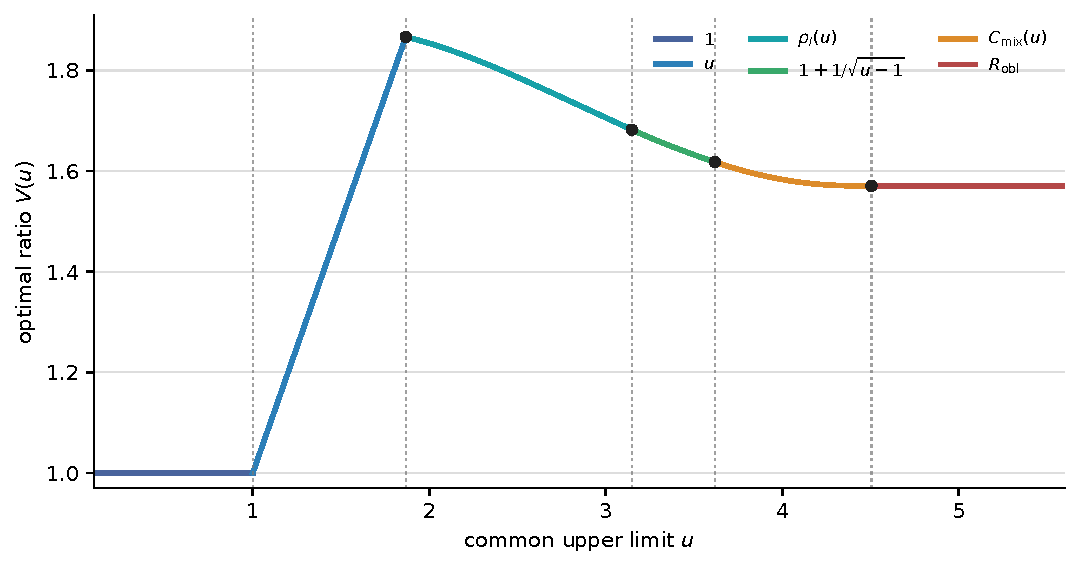
\includegraphics[width=\textwidth]{curve.pdf}
 \caption{The exact deterministic size-asymptotic ratio for finite common
 upper limit $u$.  The curve stabilizes at the obligatory endpoint value;
 dotted lines mark its five regime changes.}
 \label{fig:optional-curve}
\end{figure}

\subsection{Why total completion time leads to pair accounting}

The most useful way to think about total completion time is pairwise.  Every
operation of job $i$ contributes once to $C_i$, and it contributes once more
for each other job that remains unfinished while that operation is executed.
Equivalently, the objective consists of diagonal job terms and one delay term
for every unordered pair of jobs.  The offline pair term is simply the
shorter effective length.  The online pair term records whether an earlier
revealed job was processed immediately or left waiting.

This representation explains both sides of our proof.  A lower-bound
adversary tries to make many pairs wait in the wrong order.  An upper-bound
algorithm tries to ensure that every expensive local decision can be charged
to a corresponding offline pair.  Since there are $\Theta(n^2)$ pairs but
only $n$ diagonal terms, controlling the quadratic pair coefficient gives
the exact size-asymptotic ratio; bounded rounding errors of $O(1)$ per job
become only $O(n)$.

\subsection{Lower-bound intuition: hide the short jobs until the end}

At the obligatory endpoint, the adversary reveals equal blocks of positive
jobs from longer to shorter values and reveals a large zero block last.  The
algorithm is forced to choose between two risks.  Processing a revealed job
early may delay many still-hidden zeros.  Deferring it may leave a large tail
that delays everything completed later.  The adaptive revelation is frozen
after the interaction, so a standard replay argument produces one fixed
instance for the chosen deterministic algorithm.

The processing times are separated by harmonic gaps.  This choice is not a
guess about the final constant.  The zero mass and the number of shorter
positive blocks give two multiplicities; their sum exactly cancels the
denominator of each harmonic gap.  After this cancellation, every possible
postponement made by the algorithm has a nonnegative coefficient and every
own-phase choice contributes the same completed square.  All algorithmic
decisions disappear from the leading term.  What remains is a one-variable
ratio describing the relative positive and zero masses, and its stationary
equation is \eqref{eq:zstar}.

For finite $u$, two additional adversarial pictures appear.  When $u$ is
small or moderate, binary values $p\in\{0,u\}$ already suffice: the adversary
watches how much work the algorithm completes before revealing whether the
next jobs are zeros or caps.  For the transition to the obligatory value,
the hard instance is a capped prefix followed by a scaled copy of the
harmonic core.  The prefix exploits the optimum's ability to skip tests; the
core exploits uncertainty in the test order.  As $u$ grows, the optimal cap
mass decreases continuously to zero, leaving exactly the obligatory
construction.

\subsection{Upper-bound intuition: three policies and one common bank}
\label{sec:intro-upper-intuition}

The exact upper curve uses three simple algorithmic shapes.  Their formal
pseudocode appears later; here we describe why they are natural.

\begin{center}
\begin{tabular}{@{}p{0.24\linewidth}p{0.68\linewidth}@{}}
\toprule
approximate range & upper-bound policy at a glance \\
\midrule
$u\lesssim1.87$
 & Do not test: execute every job raw. \\
$1.87\lesssim u\lesssim3.15$
 & Test all jobs; always finish an initial fraction, then use a short/long
   threshold.  The initial fraction shrinks as $u$ grows. \\
$3.15\lesssim u\lesssim3.62$
 & Test all jobs; finish values at most one immediately and sort the rest in
   a final tail. \\
$3.62\lesssim u\lesssim4.51$
 & Use the history-dependent threshold; the proof adds a reserve for capped
   outcomes. \\
$u\gtrsim4.51$, including $\infty$
 & Use the same adaptive threshold, now with no cap reserve. \\
\bottomrule
\end{tabular}
\end{center}

\paragraph{Raw policy.}
When $u$ is very small, information costs at least as much as it can save.
The algorithm therefore runs every job raw.  Slightly beyond that trivial
range, raw execution need no longer be clairvoyantly optimal for each job,
but comparing its length $u$ with the optimum's effective lengths already
gives the first nontrivial minimax branch.

\paragraph{Forced-prefix threshold policy.}
In the next regimes the algorithm tests every job.  During an initial
fraction of the test order it processes every revealed value immediately.
After that prefix it processes only sufficiently short outcomes and sends
the rest to a shortest-processing-time tail.  The forced prefix guarantees
that some jobs finish before too many tests accumulate; the suffix threshold
protects the schedule from long revealed jobs.  As $u$ increases, the useful
prefix shrinks continuously to zero.  The algebraic branch is exactly the
point where the worst binary mixture is tangent to the target ratio; after
the prefix vanishes, balancing a capped tail against a threshold-one tail
gives the square-root branch.

\paragraph{Adaptive-threshold policy.}
For large $u$, a fixed prefix is too rigid.  The algorithm again tests jobs
in a fixed order, but its immediate-processing threshold reacts to the
observed history.  It remembers only the number $N$ of positive outcomes and
the number $D$ of those outcomes that were deferred.  A normalized balance
of the form
\[
 \frac{D-(1+c)N}{\text{number of untested jobs}}
\]
measures how much future delay has already been promised to the tail.  Near a
neutral balance the algorithm can afford to process moderately long jobs
immediately.  Every positive outcome drives the balance downward, while a
deferral refunds one unit because future tests will also delay that tail job.
When the normalized balance becomes sufficiently negative, the threshold
falls toward one.  All deferred jobs are sorted only after the tests finish.

The analysis first fixes the symbolic immediate/deferred path.  Convexity
then reduces every ordinary revealed value to one of four endpoints: a true
zero, a positive value tending to zero, the immediate side of the live
threshold, or its deferred side.  A nonnegative bank potential pays the
excess pair cost at each endpoint.  The logarithmic threshold is forced by
making the immediate and deferred boundary equations balance simultaneously;
the obligatory constant is forced by calibrating the bank's initial value.

Finite $u$ creates exactly one new endpoint: a capped value $p=u$, for which
the optimum can use raw execution and avoid the test.  On the middle bridge
this endpoint can temporarily overdraw the ordinary bank, so we add a reserve
whose balance depends only on the observed cap fraction.  At the end of the
bridge the reserve becomes zero.  With $r=\Rstar-1$, the worst residual
charge of the cap endpoint is at most $2-r(u-1)$.
The right-hand side is nonpositive precisely when
$u\ge1+2/r=\zstar$.  Thus beyond $\zstar$ the obligatory four-endpoint bank
already pays for the fifth endpoint.  The plateau in
\cref{eq:intro-plateau} is a proof-level fact, not merely a numerical
coincidence.

\subsection{Why the infinite endpoint needs a uniform proof}

For each fixed processing-time vector, the finite-$u$ offline lengths
$q_u(p)$ eventually equal $1+p$.  Nevertheless, a competitive-ratio proof
cannot blindly send $u$ to infinity: the worst instance may choose
$p\approx u$, the algorithm may depend on $u$, and the hidden constant in an
$O_u(n)$ estimate may diverge.  We avoid every such interchange.  The lower
bound uses one bounded harmonic core, which embeds in all sufficiently large
finite caps.  The high-$u$ upper bound uses one $u$-independent adaptive
algorithm and one absolute linear remainder.  Consequently the endpoint
$u=\infty$ and the finite plateau are certified by the same witnesses.

The linear remainder is lower order because
$\OPT\ge n(n+1)/2$ at $u=\infty$ and, for fixed $u$, the analogous finite
bound is also quadratic.  It implies an endpoint coefficient
$\Rstar+\eps$ with a fixed additive constant for every $\eps>0$.  We do
\emph{not} prove the stronger statement
$\ALG\le\Rstar\OPT+B$ with one fixed $B$, nor the unrelaxed inequality
$\ALG\le\Rstar\OPT$ on every finite instance.

\subsection{How to read the proofs}

After the literature review and common model, \cref{sec:obligatory} begins
with the cap-free endpoint.  Its lower subsection gives the harmonic
adversary and a reusable scaled-core lemma.  Its upper subsection formally
states the adaptive algorithm and proves the ordinary four-endpoint bank.
These are matching and may still be read independently.

\Cref{sec:optional} then treats finite caps.  The binary stopping game and
the two simple policies prove the first four branches.  The capped-prefix
lower construction reuses the harmonic core, while the middle/high upper
bound reuses the ordinary bank and analyzes only the new cap endpoint and
its reserve.  At $u=\zstar$ both cap corrections vanish.
\Cref{app:finite-checkpoint,app:cap-bubbling} contain an exact rational
checkpoint for the cap-free lower construction and an independent
cap-bubbling certificate.

\section{Related work}\label{sec:related}

Scheduling with testing belongs to the broader framework of optimization with
explorable uncertainty, where uncertain data can be queried at a cost; the
query model goes back at least to Kahan~\cite{Kahan1991}.  In the stochastic
scheduling model of Levi, Magnanti, and Shaposhnik, testing diagnoses random
job attributes and the scheduler trades the information gained against the
delay caused by diagnosis~\cite{LeviMagnantiShaposhnik2019}.  Their later work
treats heterogeneous distributions and job priorities
\cite{LeviMagnantiShaposhnik2024}.  Those policies exploit distributional
information.  The present paper instead uses worst-case processing times and
competitive analysis.

Dürr, Erlebach, Megow, and Meißner introduced the adversarial model now
usually called scheduling with testing~\cite{DurrErlebachMegowMeissner2020}.
A job has a known upper bound and may either be executed untested for that
bound or tested for one unit to reveal a possibly smaller processing time.
For total completion time on one machine they proved a deterministic lower
bound of $1.8546\ldots$ and an upper bound of $2$.  When all upper bounds are
the same, they retained the lower bound and obtained the asymptotic upper
bound $1.9338\ldots$; on the further restriction $p\in\{0,u\}$, their UTE
algorithm achieves $1.8668\ldots$.  Our finite-cap theorem closes the
common-upper gap for arbitrary $p\in[0,u]$, determines the dependence on the
fixed parameter $u$, and shows that the UTE constant is exactly the maximum
of the resulting curve.

A related binary-information model is the processing-time-oracle problem of
Dufossé et al.~\cite{DufosseEtAl2022}.  There, every job has one of two known
possible processing times and an untested execution lasts for the true
processing time; optimal adaptive and nonadaptive two-phase policies can be
computed.  This differs from our raw mode, whose duration is the declared
upper bound regardless of the hidden value.  Other variants alter a different
part of the model.  Nonuniform test times were introduced by Albers and
Eckl~\cite{AlbersEckl2021}; the competitive guarantees for that setting were
subsequently sharpened by Liu et al.~\cite{LiuLiuWongZhang2023} and, most
recently, by Krekelberg et al.~\cite{KrekelbergEtAl2026}.  Damerius et
al.~\cite{DameriusEtAl2023} place job-dependent testing costs under an
external budget, rather than charging test time directly to every unfinished
job.  Multiprocessor extensions for total completion time were studied by
Gong, Chen, and Hayashi~\cite{GongChenHayashi2024}.  Buld and
Schulz~\cite{BuldSchulz2026} recently obtained the first constant guarantees
for weighted total completion time in the adversarial optional-testing model.
These variants do not specialize to the common-upper single-machine game
solved here, but they delimit which assumptions make an exact curve possible.

Dogeas, Erlebach, and Liang introduced obligatory-test scheduling for total
completion time~\cite{DogeasErlebachLiang2024}.  For arbitrary test times,
their 1-SORT algorithm is $1.861$-competitive.  For uniform unit tests, their
fixed-threshold algorithm SIDLE processes a sufficiently short revealed job
immediately and sends longer jobs to a shortest-processing-time tail.  They
proved the upper bound $1.58451\ldots$, exhibited matching instances for
their analysis of SIDLE, and gave a $\sqrt2$ deterministic lower bound.
Liang and Liang then developed a completion-threshold framework on identical
machines; their dyadic construction improves the single-machine lower bound
to $3/2$~\cite{LiangLiang2026}.  Our harmonic multilevel construction raises
that lower bound to $\Rstar$, while the adaptive-threshold algorithm lowers
the upper bound to the same value.  Unlike SIDLE, its threshold depends on
both the number of positive outcomes observed and the number deferred.

Our pair representation is related to the delay accounting of Dogeas et
al.~\cite{DogeasErlebachLiang2024}, but the certificate is different.  Once
the immediate/deferred decisions are fixed, coordinatewise convexity reduces
the obligatory upper bound to four boundary outcomes.  A state-dependent bank
then certifies those outcomes.  The distinction between $0$ and $0^+$ forces
an extra state variable; in the finite-cap model, the endpoint $p=u$ creates
a fifth outcome because the offline optimum may skip the test.  The reserve
in \cref{sec:optional-upper} pays precisely for this cap endpoint.

For context, if processing times are revealed only when jobs finish and no
tests are available, one obtains the classical nonclairvoyant model of
Motwani, Phillips, and Torng~\cite{MotwaniPhillipsTorng1994}.  Lindermayr et
al.~\cite{LindermayrEtAl2026} instead consider online arrivals, preemption,
and total flow time when a job's operations are revealed successively.  For
their uniform two-operation specialization, operation-level SRPT is
$2$-competitive and this is tight.  That result is not directly comparable
with ours because release dates, preemption, and the flow-time benchmark all
differ.  Finally, the offline shortest-processing-time rule used below is the
unweighted special case of Smith's rule~\cite{Smith1956}.

\section{Unified model and preliminaries}\label{sec:model}

There are $n$ jobs, all available at time zero, and one machine.  Operations
are nonpreemptive, and at most one operation can run at a time.  A unit test
of job $j$ reveals its processing time $p_j\ge0$.

The family is indexed by $u\in(0,\infty]$.  For finite $u$, all jobs share
this known upper limit, $p_j\in[0,u]$, and either of two modes completes a
job: execute it untested for time $u$, or test it for one unit and
subsequently process it for time $p_j$.  An untested execution reveals no
value and needs no later test.  At the endpoint $u=\infty$, processing times
are arbitrary finite nonnegative numbers and raw execution is unavailable.
Thus every job consists of its test and a later, not necessarily immediate,
processing operation of length $p_j$.  This is exactly obligatory testing.

The completion time $C_j$ is the completion time of the processing operation;
in tested mode, when $p_j=0$, this is the instant immediately after the test.
The objective is $\sum_j C_j$.  The number $n$ and the parameter $u$ are
known to the online algorithm.

We write $\ALG_{\mathcal A}(I)$ for the objective value of an online algorithm
$\mathcal A$ on an instance $I$, and $\OPT(I)$ for the value of an offline
optimum that knows all processing times.  We omit subscripts and arguments
when they are clear.

\subsection{One offline optimum for the whole family}

Define the clairvoyant effective length by
\begin{equation}\label{eq:optional-effective-length}
 q_u(p)\defeq
 \begin{cases}
  \min\{u,1+p\},&u<\infty,\\
  1+p,&u=\infty.
 \end{cases}
\end{equation}

\begin{lemma}[Unified offline order]
\label{lem:offline}\label{lem:optional-offline}
Let $q_i=q_u(p_i)$ and let $q_{(1)}\le\cdots\le q_{(n)}$.  For every
$u\in(0,\infty]$, an offline optimum completes the jobs in nondecreasing
order of $q_i$ and has value
\begin{align}
 \OPT_u
 &=\sum_{k=1}^n\sum_{i=1}^kq_{(i)},
 \label{eq:unified-opt-prefix}\\
 &=\sum_iq_i+\sum_{i<j}\min\{q_i,q_j\}.
 \label{eq:optional-opt-pair}
\end{align}
For finite $u$, it uses raw mode when $u\le1+p_j$ and tested mode otherwise.
At $u=\infty$, it tests every job and processes the jobs in nondecreasing
$p_j$ order.
\end{lemma}

\begin{proof}
Let $C_{[1]}\le\cdots\le C_{[n]}$ be the completion times of any feasible
schedule.  Completing job $j$ consumes at least $q_j$ units: for finite $u$
this is the shorter of its two modes, and for $u=\infty$ it is its compulsory
test--process length.  By time $C_{[k]}$ the machine has completed some $k$
jobs, so
\[
 C_{[k]}\ge\sum_{i=1}^kq_{(i)}.
\]
The schedule that takes the shorter available mode for every job and executes
the resulting blocks in nondecreasing $q_i$ order attains every inequality.
Summing and expanding the prefix sums gives both formulas.
\end{proof}

At the cap-free endpoint, the pair formula specializes to
\begin{align}
 \OPT_\infty
 &=\sum_{k=1}^n\left(k+\sum_{i=1}^kp_{(i)}\right),
 \label{eq:opt-prefix}\\
 &=\sum_i(1+p_i)+\sum_{i<j}\bigl(1+\min\{p_i,p_j\}\bigr).
 \label{eq:opt-pair}
\end{align}
In particular,
\begin{equation}\label{eq:opt-n2}
 \OPT_\infty\ge\frac{n(n+1)}2.
\end{equation}
For finite $u$, $q_j\ge\min\{u,1\}$ gives
\begin{equation}\label{eq:optional-opt-n2}
 \OPT_u\ge\min\{u,1\}\frac{n(n+1)}2.
\end{equation}

\subsection{Competitive-ratio conventions}

The ordinary competitive ratio of $\mathcal A$ is
\[
  \CR(\mathcal A)=\sup_I\frac{\ALG_{\mathcal A}(I)}{\OPT(I)}.
\]
For the result of this paper, the relevant size-asymptotic ratio is
\begin{equation}\label{eq:cr-infty}
  \CR_\infty(\mathcal A)
  =\limsup_{n\to\infty}\ \sup_{|I|=n}
       \frac{\ALG_{\mathcal A}(I)}{\OPT(I)}.
\end{equation}
The additive-constant convention calls a coefficient $c$ admissible for
$\mathcal A$ if there exists $B<\infty$ such that
\[
  \ALG_{\mathcal A}(I)\le c\OPT(I)+B
  \qquad\text{for every }I.
\]
We write
\begin{equation}\label{eq:cr-add}
  \CR_{\rm add}(\mathcal A)
  =\inf\{c:\text{$c$ is admissible for $\mathcal A$}\}.
\end{equation}
The optimal deterministic values in the two conventions are obtained by
taking the infimum of $\CR_\infty(\mathcal A)$ and
$\CR_{\rm add}(\mathcal A)$, respectively, over deterministic algorithms.
For any fixed $u$, an estimate $\ALG\le c\OPT+O_u(n)$ fixes
\cref{eq:cr-infty} at most $c$ and, by
\cref{eq:opt-n2,eq:optional-opt-n2}, makes every coefficient $c+\eps$
admissible.  It need not make the endpoint coefficient $c$ admissible.

\begin{remark}[No hidden interchange of limits]\label{rem:no-limit-swap}
The notation $u=\infty$ identifies one model exactly.  We never infer an
endpoint upper bound merely by taking $u\to\infty$ in an estimate whose
algorithm or additive term may depend on $u$.  The endpoint estimate is
proved directly in \cref{sec:upper}; \cref{sec:optional-upper} then verifies
that the same algorithm and certificate work uniformly for every finite
$u\ge\zstar$.
\end{remark}

\subsection{Test-order adversaries}

The lower bound will assign processing times according to the order in which
tests finish.  This is only a proof device.

\begin{lemma}[Replay]\label{lem:replay}
Fix a deterministic online algorithm.  Suppose all untested jobs have the
same known parameters, and an adversary assigns processing times
deterministically from the transcript and test-completion order.  The
resulting interaction is reproduced by a fixed input instance.
\end{lemma}

\begin{proof}
Run the interaction once and record the value revealed for every tested job
label.  Assign those values to the corresponding labels in advance.  An
induction over operation completions shows that the deterministic algorithm
chooses the same tests, processing operations, and idle intervals on the fixed
instance.  If the algorithm fails to test or complete some job forever, its
competitive ratio is already infinite; otherwise every relevant label is
recorded.
\end{proof}

\section{The cap-free endpoint \texorpdfstring{$u=\infty$}{u=infinity}}
\label{sec:obligatory}

This section contains the two estimates needed for the cap-free endpoint
theorem and isolates the harmonic and four-endpoint cores reused later.
The first subsection applies to an arbitrary deterministic online algorithm;
the second analyzes one explicit algorithm.  Each restates the local notation
it uses.

\subsection{The cap-free harmonic core}
\label{sec:lower}

This subsection develops the cap-free construction used by the last two
branches of the revealing curve.  Its notation is local to this subsection.
We first record its extremal specialization and then extract the scaled form
reused by the mixed branch.  The construction
has many equally large groups of positive jobs, revealed from longest to
shortest, followed by one large group of zero jobs.  The only design choice is
the gap between two consecutive positive processing times.  Choosing these
gaps harmonically will make all decisions of the online algorithm disappear
from the leading term.

\begin{theorem}[Extremal harmonic core]
\label{thm:lower}
For every deterministic online algorithm $\mathcal B$ and every $\eps>0$,
there are arbitrarily large fixed instances $I$ with unit tests and rational
processing times such that
\[
  \ALG_{\mathcal B}(I)\ge (\RdetOT-\eps)\OPT(I).
\]
\end{theorem}

\paragraph{The revelation experiment.}
Fix an integer $K$, a rational number $\xi>0$, and a rational slack
$\gamma\in(0,1)$; one may keep $\gamma=1/2$ throughout.  For a large scaling
integer $H$, the instance will contain $H$ jobs of each of $K$ positive types
$0,1,\ldots,K-1$ and $\xi H$ zero jobs.  We choose $H$ to clear all
denominators.

The adversary assigns processing times according to the order in which tests
are started.  The first $H$ tested jobs receive processing time $p_0$, the
next $H$ receive $p_1$, and so on; after the $K$ positive blocks, every
remaining job receives processing time zero.  Thus
\[
  p_0>p_1>\cdots>p_{K-1}>1,
\]
so the algorithm sees the positive types from longest to shortest and learns
about the zero jobs only at the end.

This adaptive description is only a convenient way to construct the input.
After running the interaction against a fixed deterministic algorithm, assign
to every job label the value revealed when that label was tested.  Replaying
the algorithm on this fixed assignment produces exactly the same transcript.
If the algorithm never tests or completes some job, its cost is infinite and
the lower bound is immediate; otherwise every job label is recorded.
Hence it is enough to lower-bound the cost in the revelation experiment.

\paragraph{Why each phase can be relaxed to shortest processing time.}
Let $T_\ell$ be the start of the first test in positive block $\ell$, and let
$T_K$ be the start of the first test in the zero block.  Phase $\ell$ contains
the completions in $(T_\ell,T_{\ell+1}]$; a completion exactly at $T_\ell$
belongs to the preceding phase.  Each $T_\ell$ is the boundary between two
nonpreemptive operations.  Consequently, a previously tested job that is
unfinished at $T_\ell$ has not started processing and still needs its entire
processing time.

We repeatedly use the following elementary observation.  Suppose jobs with
remaining work $v_1,\ldots,v_m$ complete after some time $T$.  If their
completion order is $q_1,\ldots,q_m$, then the $r$th relative completion time
is at least $\sum_{h\le r}v_{q_h}$.  Summing these prefix inequalities shows
that their total relative completion time is minimized by arranging the
$v_i$ in nondecreasing order.  This is merely a lower bound; the online
algorithm need not actually use that order.

For normalized group masses $q_1,\ldots,q_m$ and remaining lengths
$v_1\le\cdots\le v_m$, this shortest-first bound has leading coefficient
\begin{equation}
 \mathcal S((q_g,v_g)_{g=1}^m)
 =\sum_{g=1}^m
   \left(\frac{v_gq_g^2}{2}
    +q_g\sum_{h<g}v_hq_h\right).
 \label{eq:lower-S}
\end{equation}
More precisely, the corresponding contribution for groups of size $q_gH$
is $H^2\mathcal S+O(H)$.  The quadratic term is simply the familiar sum
$v_g(1+\cdots+q_gH)$ inside one group; the cross term is the waiting caused
by all shorter groups.

We ensure that
\begin{equation}
  p_0-p_{K-1}<1.
  \label{eq:lower-span}
\end{equation}
In phase $\ell$, an unfinished job of an older type $j<\ell$ therefore has
remaining length $p_j$, whereas a type-$\ell$ job completed in its own phase
needs both its test and processing, of total length $1+p_\ell$.  Their order
in the shortest-first relaxation is
\[
  p_{\ell-1}<p_{\ell-2}<\cdots<p_0<1+p_\ell.
\]
At $T_K$, an untested zero job has remaining length $1$, so the relaxed tail
starts with all zero jobs and then uses the positive types from shortest to
longest.  These are the only two places where
\cref{eq:lower-span} is used.

\paragraph{The finite accounting identity.}
We now record the online algorithm's possible behavior.  Normalize all job
counts by $H$.  Let
\begin{itemize}
\item $s_j\in[0,1]$ be the mass of type-$j$ jobs completed in their own
      phase;
\item $d_{j,\ell}\ge0$ be the mass of type-$j$ jobs completed in the later
      phase $\ell>j$; and
\item
\[
  X_{j,\ell}=s_j+\sum_{r=j+1}^{\ell-1}d_{j,r}\le1
  \qquad(\ell>j)
\]
be the mass of type $j$ completed before phase $\ell$.  Thus
$X_{j,\ell+1}$ is the mass completed by the end of phase $\ell$.
\end{itemize}
At time $T_\ell$, the machine has already performed the tests of the $\ell H$
jobs in earlier positive blocks and has processed every earlier job that has
completed.  Thus
\begin{equation}
  \frac{T_\ell}{H}
  \ge \ell+\sum_{j<\ell}p_jX_{j,\ell}.
  \label{eq:lower-start}
\end{equation}
For each phase, charge its completions their common start time from
\cref{eq:lower-start}, and charge their relative completion times using
\cref{eq:lower-S}.  Do the same at $T_K$ for the remaining positive jobs
and the $\xi H$ zero jobs.  Expanding and collecting equal variables gives
\begin{align}
 \frac{\ALG}{H^2}
 \ge{}& C_K
 +\sum_{j=0}^{K-1}\left(\frac{s_j^2}{2}-\theta_js_j\right)
 \nonumber\\
 &+\sum_{j<\ell}d_{j,\ell}
 \left[
   \ell-j-\theta_j
   -\sum_{j<k<\ell}(p_j-p_k)X_{k,\ell+1}
 \right]-O(1/H),
 \label{eq:lower-accounting}
\end{align}
where $K,\xi,\gamma$ are fixed while $H\to\infty$, and
\begin{align}
 \theta_j
   &=1-\xi(p_j-1)-\sum_{k>j}(p_j-p_k-1),
   \label{eq:lower-theta}\\
 C_K
   &=\frac{\xi^2}{2}+2\xi K+K^2+P_K,
 &
 P_K&=\sum_{j=0}^{K-1}\left(j+\frac12\right)p_j.
 \label{eq:lower-CP}
\end{align}

For completeness, here is how to audit
\cref{eq:lower-accounting} without guessing its origin.  In phase $\ell$,
the masses in the shortest-first relaxation are
\[
 d_{\ell-1,\ell},d_{\ell-2,\ell},\ldots,d_{0,\ell},s_\ell
\]
with respective lengths
\[
 p_{\ell-1},p_{\ell-2},\ldots,p_0,1+p_\ell.
\]
Multiply their total mass by the right-hand side of
\cref{eq:lower-start} and add the functional
\cref{eq:lower-S}.  In the final phase use masses
\[
 \xi,\ 1-X_{K-1,K},\ldots,1-X_{0,K}
\]
and lengths $1,p_{K-1},\ldots,p_0$.  The constant terms sum to $C_K$.
The terms containing only $s_j$ are $s_j^2/2-\theta_js_j$; the coefficient
of each $d_{j,\ell}$ is precisely the bracket in
\cref{eq:lower-accounting}.  Thus the displayed identity is just the
phasewise shortest-first bound with the phase start times retained.  No
optimality assumption about the online schedule is hidden in it.

The meaning of the expression is useful.  Completing an $s_j$ fraction of a
type in its own phase creates a quadratic completion cost but saves later
waiting cost, producing $s_j^2/2-\theta_js_j$.  A completion postponed to a
later positive phase is represented by $d_{j,\ell}$ and its bracket.  We next
choose the processing times so that every such bracket is nonnegative and all
$\theta_j$ are equal.

\paragraph{The harmonic choice and its telescoping cancellation.}
Set
\begin{equation}
  p_{K-1}=1+\frac{\gamma}{\xi},
  \qquad
  p_i=p_{i+1}+\frac1{\xi+K-1-i}
  \quad(0\le i<K-1).
  \label{eq:lower-harmonic}
\end{equation}
In other words, measured upward from the shortest type, the consecutive gaps
are
\[
  \frac1{\xi+1},\frac1{\xi+2},\ldots,\frac1{\xi+K-1}.
\]
This is the key design choice.  If $m=K-1-j$, then
\begin{align*}
 p_j-1
   &=\frac\gamma \xi+\sum_{r=1}^m\frac1{\xi+r},\\
 \sum_{k>j}(p_j-p_k)
   &=\sum_{r=1}^m\frac{r}{\xi+r}.
\end{align*}
Adding the first line multiplied by $\xi$ to the second line makes each
denominator cancel:
\begin{equation}
 \xi(p_j-1)+\sum_{k>j}(p_j-p_k)
 =\gamma+\sum_{r=1}^m\frac{\xi+r}{\xi+r}
 =\gamma+m.
 \label{eq:lower-telescope}
\end{equation}
Substitution in \cref{eq:lower-theta} gives the same value for every type,
\begin{equation}
  \theta_j=1-\gamma.
  \label{eq:lower-theta-constant}
\end{equation}
This is why the increments in \cref{eq:lower-harmonic} are harmonic: the
factor $\xi$ coming from the zero block and the multiplicity $r$ coming from the
$r$ shorter positive types add up to the denominator $\xi+r$.

The delayed-completion terms are now harmless as well.  Since
$X_{k,\ell+1}\le1$, their brackets are at least
\begin{align*}
 &\ell-j-(1-\gamma)
   -\sum_{j<k<\ell}(p_j-p_k)\\
 &\hspace{20mm}
 =\gamma+\sum_{j<k<\ell}\bigl(1-(p_j-p_k)\bigr)>0,
\end{align*}
where the final inequality follows from
\cref{eq:lower-span}.  We may therefore drop every term containing
$d_{j,\ell}$.  The remaining minimization is not a multivariable optimization
problem: complete one square for each $j$,
\[
  \frac{s_j^2}{2}-(1-\gamma)s_j
  =\frac12\bigl(s_j-(1-\gamma)\bigr)^2
   -\frac12(1-\gamma)^2.
\]
Because $1-\gamma\in(0,1)$, this minimum is feasible for
$s_j\in[0,1]$.  Hence every online algorithm obeys
\begin{equation}
 \liminf_{H\to\infty}\frac{\ALG}{H^2}
 \ge Q_K
 \defeq C_K-\frac K2(1-\gamma)^2.
 \label{eq:lower-QK}
\end{equation}

It remains to compute the offline benchmark.  Knowing all processing times,
the optimum runs the zero jobs first and the positive types from shortest to
longest.  Equivalently, the pairwise contribution of two jobs is
$1+\min\{p_i,p_j\}$.  Its leading coefficient is
\begin{equation}
  D_K=\frac{\xi^2}{2}+\xi K+\frac{K^2}{2}+P_K,
  \qquad
  \lim_{H\to\infty}\frac{\OPT}{H^2}=D_K.
  \label{eq:lower-DK}
\end{equation}
The four terms respectively account for zero--zero pairs, zero--positive
pairs, the unit-test part of positive--positive pairs, and the processing
part of positive--positive pairs.  Thus the finite-$K$ lower-bound
certificate is simply $Q_K/D_K$.

\paragraph{Passing to a smooth curve.}
Write
\[
  \alpha=\frac K\xi
\]
for the ratio of positive mass to zero mass, and keep $\alpha$ fixed while
$K\to\infty$.  We restrict to $0<\alpha<e-1$.  Then
\[
 p_0-p_{K-1}
 =\sum_{r=1}^{K-1}\frac1{\xi+r}
 <\ln\!\left(1+\frac K\xi\right)
 =\ln(1+\alpha)<1,
\]
which verifies \cref{eq:lower-span}.

The processing contribution $P_K$ has the exact form
\begin{equation}
 P_K
 =\frac{K^2}{2}\left(1+\frac\gamma \xi\right)
  +\frac12\sum_{h=1}^{K-1}\frac{(K-h)^2}{\xi+h}.
 \label{eq:lower-P-exact}
\end{equation}
Indeed, the common baseline $1+\gamma/\xi$ contributes the first term, and
swapping the order of summation shows that the increment $1/(\xi+h)$ receives
total weight $(K-h)^2/2$.  After division by $\xi^2$, the sum becomes a
Riemann integral:
\begin{align}
 \frac{P_K}{\xi^2}&\longrightarrow I(\alpha)
   =\frac{\alpha^2}{2}
    +\frac12\int_0^\alpha\frac{(\alpha-t)^2}{1+t}\,dt
   \nonumber\\
 &=\int_0^\alpha(\alpha-t)\bigl(1+\ln(1+t)\bigr)\,dt
   \nonumber\\
 &=\frac12(1+\alpha)^2\ln(1+\alpha)
   -\frac\alpha2-\frac{\alpha^2}{4}.
 \label{eq:lower-I}
\end{align}
The second integral form follows either by integration by parts or by summing
the limiting processing-time curve $1+\ln(1+t)$ against the remaining
positive mass $\alpha-t$.
The subtraction in \cref{eq:lower-QK} is only $O(K)$, whereas
$C_K,D_K=\Theta(K^2)$.  Since $C_K-D_K=\xi K+K^2/2$, we obtain
\begin{equation}
 R(\alpha)
 \defeq\lim_{K\to\infty}\frac{Q_K}{D_K}
 =1+
 \frac{\alpha+\alpha^2/2}
 {\frac12+\frac\alpha2+\frac{\alpha^2}{4}
  +\frac12(1+\alpha)^2\ln(1+\alpha)}.
 \label{eq:lower-Ralpha}
\end{equation}

This last one-variable maximization is where the constant in the theorem
comes from.  Put $z=(1+\alpha)^2$.  Then
\begin{equation}
  R(z)=1+\frac{2(z-1)}{1+z+z\ln z}.
  \label{eq:lower-Rz}
\end{equation}
The derivative of the fraction has the sign of
\[
  3-z+\ln z.
\]
For $z>1$ this expression is strictly decreasing, is positive at $z=1$, and
tends to $-\infty$.  Hence it has one zero $\zstar$, characterized by
\[
  \zstar-3=\ln \zstar.
\]
The derivative is positive before $\zstar$ and negative afterward, so this is
the global maximum.  At the root,
\[
  1+\zstar+\zstar\ln \zstar=(\zstar-1)^2,
\]
and therefore
\[
  R(\zstar)=1+\frac{2}{\zstar-1}=\RdetOT.
\]
Moreover, $\sqrt{\zstar}-1=1.12255\ldots<e-1$, so the maximizer lies in the
range where \cref{eq:lower-span} holds.

\begin{proof}[Proof of \cref{thm:lower}]
Choose a rational $\alpha$ sufficiently close to
$\alpha_\star=\sqrt{\zstar}-1$, and choose any rational
$\gamma\in(0,1)$.  For a sufficiently large $K$, set $\xi=K/\alpha$ and use
\cref{eq:lower-harmonic}; then $Q_K/D_K>\RdetOT-\eps/2$.
All parameters are rational.  Let $H$ tend to infinity through multiples of
their common denominators.  \Cref{eq:lower-QK,eq:lower-DK} make the actual ratio exceed
$\RdetOT-\eps$ for all sufficiently large $H$.  Finally, the replay argument
at the beginning of the proof converts the revelation experiment into a fixed
instance for the given deterministic algorithm.
\end{proof}

\begin{lemma}[Scaled harmonic core]
\label{lem:opt:harmonic-block}
Fix a total normalized mass $s>0$ and a parameter $t\in[1,e)$.  Against
every deterministic obligatory-testing algorithm, there are scales
$M_\nu\to\infty$ and finite rational multilevel instances with
$sM_\nu+o(M_\nu)$ jobs such that
\begin{equation}
 \frac{\OPT}{M_\nu^2}\longrightarrow
 O_0=\frac{s^2}{4}(1+t^{-2}+2\ln t),
 \qquad
 \liminf_{\nu\to\infty}\frac{\ALG}{M_\nu^2}
 \ge A_0^{\rm lb}
 \defeq O_0+\frac{s^2}{2}(1-t^{-2}).
 \label{eq:opt:harmonic-coefficients}
\end{equation}
Their normalized total positive processing mass converges to
\begin{equation}
 \frac1{M_\nu}\sum_{j:p_j>0}p_j\longrightarrow L=s\ln t,
 \label{eq:opt:harmonic-processing-mass}
\end{equation}
and their largest processing time converges to $1+\ln t<2$.
The adaptive revelation is converted by replay into a fixed instance.
\end{lemma}

\begin{proof}
The case $t=1$ is obtained by continuity from instances with vanishing
positive mass, so suppose $1<t<e$.  In the construction above set
$\alpha=t-1=K/\xi$.  Before rescaling, the total normalized mass is
$K+\xi=\xi t$.  Give every unit of normalized mass the common factor
$s/(\xi t)$.

The phase accounting, harmonic cancellation, and completion of squares in
\cref{eq:lower-accounting,eq:lower-telescope,eq:lower-QK} are homogeneous of
degree two in the job masses.  The Riemann-sum limit
\cref{eq:lower-I} substituted into \cref{eq:lower-DK} therefore gives
\[
 O_0=\frac{s^2}{4}(1+t^{-2}+2\ln t).
\]
Likewise $C_K-D_K=\xi K+K^2/2$, while the $O(K)$ square-completion loss in
\cref{eq:lower-QK} disappears after division by the quadratic scale.  After
the same rescaling this gives the guaranteed lower benchmark
\[
 A_0^{\rm lb}-O_0=\frac{s^2}{2}(1-t^{-2}).
\]
Finally, summing the limiting processing-time curve
$1+\ln(1+x)$ over the positive mass gives $L=s\ln t$, and
\cref{eq:lower-harmonic} gives $p_0\to1+\ln t$.  Rational approximation,
clearing denominators, and the replay argument used in the theorem produce a
diagonal sequence of arbitrarily large fixed rational instances with the
stated limit and liminf bounds.
\end{proof}


\subsection{Upper bound: a self-contained proof}
\label{sec:upper}

We prove the following statement from scratch in this subsection.

\begin{theorem}[Upper bound]
\label{thm:upper}
Let $z>1$ be the solution of $z-3=\log z$, and set
\[
 R=1+\rho,
 \qquad
 \rho=\frac{2}{z-1}=0.5705740966\ldots .
\]
There is a deterministic online algorithm and an absolute constant $C$ such
that every instance with $n$ jobs satisfies
\[
  \ALG\le R\OPT+Cn.
\]
\end{theorem}

The proof has three ingredients.  First, pairwise accounting gives an exact
formula for the cost of a schedule.  Second, a simple convexity argument says
that it is enough to consider four boundary outcomes for every test.  Third,
we give a nonnegative \emph{bank balance} $W$: whenever a boundary outcome
creates positive excess cost, the balance drops by at least that amount, up
to a constant rounding loss.  Thus the proof below uses derivatives only as
shorthand for the first-order change of this bank balance; no optimization
background is needed.

\paragraph{The algorithm.}
For a parameter $c>0$, the formal procedure
\textsc{AdaptiveThreshold}$(c)$ is given in
\cref{alg:adaptive-threshold}.  Immediately before a test, let
\begin{itemize}
\item $x$ be the number of jobs not yet tested, including the job about to be
      tested;
\item $N$ be the number of earlier tests that revealed a strictly positive
      processing time; and
\item $D$ be the number of these $N$ jobs that the algorithm deferred.
\end{itemize}
Define the normalized state
\begin{equation}
\label{eq:upper-y}
 y=\frac{D-RN}{x}.
\end{equation}
Because $D\le N$ and $R>1$, we always have $y\le0$.  For later reuse define
the parameterized threshold
\begin{equation}
\label{eq:upper-A}
 a_c(y)=
 \begin{cases}
  1, & y\le-1,\\[1mm]
  \displaystyle
  1+\frac12\log\!\left(\frac{c+2}{c-2y}\right),
       & -1\le y\le0.
 \end{cases}
\end{equation}
The theorem uses $c=\rho$; throughout this subsection we abbreviate
$A(y)=a_\rho(y)$ and $R=1+\rho$.
The defining equation for $z=(\rho+2)/\rho$ says
\begin{equation}
\label{eq:upper-root-rho}
 \log\frac{\rho+2}{\rho}=\frac2\rho-2.
\end{equation}
Consequently, $A$ is continuous at $-1$, increases from $A(-1)=1$ to
$A(0)=1/\rho=1.7526207478\ldots$, and
\begin{equation}
\label{eq:upper-A-prime}
 A'(y)=\frac{1}{\rho-2y}
 \qquad (-1<y<0).
\end{equation}

\begin{algorithm}[H]
\caption{\textsc{AdaptiveThreshold}$(J,c)$}
\label{alg:adaptive-threshold}
\begin{algorithmic}
\Statex \textbf{Input:} jobs $J$ and parameter $c>0$.
\State Fix an arbitrary test order $j_1,\ldots,j_n$.
\State Set $N\gets0$, $D\gets0$, and $Q\gets\varnothing$.
\State \textbf{For} $i=1,\ldots,n$ \textbf{do}:
\State \quad Set $x\gets n-i+1$ and $y\gets(D-(1+c)N)/x$.
\State \quad Set $a\gets a_c(y)$ according to \cref{eq:upper-A}.
\State \quad Test $j_i$ for one unit and observe $p_{j_i}$.
\State \quad \textbf{If} $p_{j_i}\le a$, process $j_i$ immediately.
\State \quad \textbf{Otherwise}, add $j_i$ to $Q$ and set $D\gets D+1$.
\State \quad \textbf{If} $p_{j_i}>0$, set $N\gets N+1$.
\State Process the jobs of $Q$ in nondecreasing order of their revealed
       processing times.
\end{algorithmic}
\end{algorithm}

For $c=\rho$, the state in the pseudocode is exactly
\eqref{eq:upper-y}.  A genuine zero increments neither counter and completes
at the end of its test.  The procedure never uses raw execution; the same
pseudocode will therefore apply to the large finite-$u$ regimes.

The numerator $D-RN$ in \eqref{eq:upper-y} is best viewed as a balance,
not as an estimate of a processing time.  Every revealed positive job reduces
the balance by $R$; deferring it returns one unit, because every later unit
test will also delay that deferred job.  Dividing by $x$ spreads this balance
over the tests that remain.  A state close to $0$ can afford a threshold
larger than one.  Once the normalized balance falls below $-1$, the proof can
only support the conservative threshold one, so $A$ becomes flat.

We will later derive \eqref{eq:upper-A}, rather than asking the reader to
guess why this particular logarithm appears.

\paragraph{Pairwise accounting.}
For two jobs $i<j$ in test order, charge to their unordered pair the duration
of operations of either job performed while the other job is unfinished.  If
job $i$ is processed immediately, this charge in the algorithm is $1+p_i$.
If $i$ is deferred and $j$ is immediate, it is $2+p_j$.  If both are
deferred, it is $2+\min\{p_i,p_j\}$.  Hence
\begin{equation}
\label{eq:upper-alg-pair}
 \ALG=\sum_i(1+p_i)+\sum_{i<j}g_{ij},
 \qquad
 g_{ij}=
 \begin{cases}
  1+p_i, & i\text{ immediate},\\
  2+p_j, & i\text{ deferred},\ j\text{ immediate},\\
  2+\min\{p_i,p_j\}, & i,j\text{ deferred}.
 \end{cases}
\end{equation}
The offline optimum tests and immediately processes jobs in nondecreasing
order of $p_i$, and therefore
\begin{equation}
\label{eq:upper-opt-pair}
 \OPT=\sum_i(1+p_i)
       +\sum_{i<j}\bigl(1+\min\{p_i,p_j\}\bigr).
\end{equation}
For completeness, the latter claim follows because the $k$th completed job
cannot finish before the machine has performed $k$ tests and the processing
of the $k$ shortest jobs.  The shortest-first schedule attains all these
lower bounds simultaneously.

We bound the excess
\[
 F=\ALG-R\OPT.
\]

\paragraph{Why four boundary outcomes suffice.}
Fix only the symbolic decisions made along a run: for each job, specify
whether its value is zero, positive and immediate, or positive and deferred.
This fixes all later counters and thresholds.  The allowed values of a
coordinate are then, respectively,
\[
 \{0\},\qquad (0,A(y)],\qquad (A(y),\infty).
\]
If all processing times except $p_i$ are fixed inside such a symbolic run,
\eqref{eq:upper-alg-pair}--\eqref{eq:upper-opt-pair} express $F$ as an
affine function of $p_i$ plus negative multiples of
$\min\{p_i,h\}$.  Since $p\mapsto\min\{p,h\}$ is concave, $F$ is convex in
$p_i$.  A convex function on $(0,A(y)]$ has its supremum at one of the two
ends.  On $(A(y),\infty)$, the eventual slope is $1-R=-\rho<0$; convexity
then implies that every earlier slope is also negative, so the supremum is at
the lower end.

It is therefore enough to consider the following four formal outcomes.
\begin{center}
\begin{tabular}{ccll}
\toprule
type & limiting value & algorithmic decision & counter update\\
\midrule
$\mathsf Z$ & $0$ & immediate & none\\
$\mathsf E$ & $0^+$ & immediate & $N\leftarrow N+1$\\
$\mathsf I$ & $A(y)$ & immediate & $N\leftarrow N+1$\\
$\mathsf Q$ & $A(y)^+$ & deferred
             & $N\leftarrow N+1$, $D\leftarrow D+1$\\
\bottomrule
\end{tabular}
\end{center}
Here $0^+$ is not a new processing time.  It means that a positive immediate
value tends to zero \emph{after its symbolic decision has been fixed}.
Although its processing contribution vanishes, it still increments $N$ and
therefore changes all future thresholds.  This is why $0$ and $0^+$ cannot be
identified.  Similarly, $A(y)^+$ approaches the threshold from the deferred
side.  Applying the one-coordinate argument successively shows that a uniform
bound on all formal four-type words implies the same bound on all genuine
instances.  Because $F$ is a finite sum of affine and minimum terms on a fixed
symbolic path, the simultaneous one-sided limit at every formal vertex exists
and is independent of the rates at which its open coordinates approach their
endpoints.

One more elementary property will simplify every minimum in the pairwise
formulas.  Put $u=D-RN\le0$.  After an outcome of type $\mathsf Z$,
$\mathsf E$ or $\mathsf I$, or $\mathsf Q$, respectively, the pair $(u,x)$
changes as follows:
\[
 (u,x-1),\qquad (u-R,x-1),\qquad (u-R,x-1),\qquad
 (u-\rho,x-1).
\]
Whenever $x\ge2$, the new quotient is at most $u/x$.  Thus the states, and
hence the thresholds, seen by successive tests never increase.  When $x=1$
there is no next test and therefore no next threshold to compare.  The
nonzero boundary values $A(y)$ consequently arrive in nonincreasing order.
In particular, the minimum of the current nonzero boundary value and any
earlier one is always the current value.

\paragraph{The proof state and the local excess.}
The algorithm needs only $(x,N,D)$.  The analysis splits $N$ into two kinds.
Among earlier formal outcomes, let
\begin{itemize}
\item $S$ be the number of \emph{substantive} positive outcomes
      $\mathsf I,\mathsf Q$;
\item $e$ be the number of infinitesimal outcomes $\mathsf E$; and
\item $d$ be the number of deferred outcomes $\mathsf Q$.
\end{itemize}
Thus $N=S+e$ and $D=d$.  Define
\begin{equation}
\label{eq:upper-eta-b}
 \eta=\frac{d-RS}{x},
 \qquad
 b=\frac e x,
 \qquad
 y=\eta-Rb.
\end{equation}
We have $d\le S$, hence $\eta\le0$.  The variable $b$ records exactly the
part of the algorithmic state that is invisible to limiting processing-cost
minima: an infinitesimal value affects $N$, but its minimum with every other
processing time tends to zero.

Consider the current boundary outcome at a pre-state $(x,S,e,d)$, and write
$a=A(y)$.  Pairwise accounting gives
\begin{equation}
\label{eq:upper-exact-decomposition}
 F=-\rho\frac{n(n+1)}2+\sum_i\widetilde\ell_i,
\end{equation}
where the exact contribution of the current outcome is
\begin{align}
 \widetilde\ell_{\mathsf Z}
 =\widetilde\ell_{\mathsf E}&=d,\label{eq:upper-exact-ZE}\\
 \widetilde\ell_{\mathsf I}
 &=d+a[x+d-RS-R],\label{eq:upper-exact-I}\\
 \widetilde\ell_{\mathsf Q}
 &=d+a[d-RS-\rho].\label{eq:upper-exact-Q}
\end{align}
Here is a quick derivation.  The current unit test gives one extra unit of
algorithmic pair cost for each earlier deferred job, producing $d$.  Its own
test and its pairs with all earlier jobs give a universal excess
$-\rho(i+1)$ at step $i$; summing this term produces the first term in
\eqref{eq:upper-exact-decomposition}.  For an $\mathsf I$ outcome, the
current processing operation contributes $a(x+d)$ to the algorithm and
$Ra(S+1)$ to the scaled optimum.  For a $\mathsf Q$ outcome, the corresponding
quantities are $a(d+1)$ and $Ra(S+1)$.  Monotonicity of the thresholds justifies
using the current $a$ in every earlier processing-time minimum.

For the potential calculation it is convenient to discard the two favorable
diagonal terms $-Ra$ and $-\rho a$.  Define the relaxed local rewards
\begin{align}
 \ell_{\mathsf Z}=\ell_{\mathsf E}&=d,\label{eq:upper-ell-ZE}\\
 \ell_{\mathsf I}&=d+a(x+d-RS)
                  =d+ax(1+\eta),\label{eq:upper-ell-I}\\
 \ell_{\mathsf Q}&=d+a(d-RS)
                  =d+ax\eta.\label{eq:upper-ell-Q}
\end{align}
Then $\widetilde\ell_c\le\ell_c$ for all four types, and
\begin{equation}
\label{eq:upper-F-relaxed}
 F\le-\rho\frac{n(n+1)}2+\sum_i\ell_i.
\end{equation}

\paragraph{How the logarithmic threshold is found.}
Before giving the full bank balance, it is useful to see where the formula
comes from.  Ignore $0^+$ outcomes for a moment, so $b=0$, and look in the
range $-1\le y\le0$.  Suppose the nonlinear part of the balance has the form
$x^2f(y)$.  Asking the immediate boundary $\mathsf I$ and the deferred
boundary $\mathsf Q$ to be exactly paid by the first-order decrease of this
balance gives
\begin{align}
 -2f+(y-R)f'+A(1+y)&=0,\label{eq:upper-design-I}\\
 1-2f+(y-\rho)f'+Ay&=0.\label{eq:upper-design-Q}
\end{align}
Subtracting the equations gives $f'=A-1$.  Differentiating either equation
then gives
\[
 1+(2y-\rho)A'(y)=0.
\]
With the natural joining condition $A(-1)=1$, this is exactly
\eqref{eq:upper-A}--\eqref{eq:upper-A-prime}.

The universal negative term in \eqref{eq:upper-F-relaxed} has leading
part $-\rho n^2/2$.  The initial balance will be $n^2f(0)$, so exact
cancellation requires $f(0)=\rho/2$.  Since
\begin{equation}
\label{eq:upper-f-definition}
 f(y)=\int_{-1}^{y}(A(t)-1)\,dt,
\end{equation}
direct integration gives
\[
 f(0)=\frac12-\frac{\rho}{4}
       \log\!\left(\frac{\rho+2}{\rho}\right).
\]
Thus $f(0)=\rho/2$ is equivalent to
\eqref{eq:upper-root-rho}, or, after setting $z=(\rho+2)/\rho$, to
$z-3=\log z$.  Thus both the threshold and the constant $R$ are forced by
two local balance equations and the initial accounting; they are not the
output of an unexplained numerical optimization.

\paragraph{The bank balance.}
For $-1\le y\le0$, put
\begin{equation}
\label{eq:upper-fh}
 f(y)=\int_{-1}^{y}(A(t)-1)\,dt,
 \qquad
 h(y)=A(y)(1+y).
\end{equation}
The term $x d$ in the balance below pays for the fact that each of the $x$
remaining tests will delay each of the $d$ already deferred jobs.  The
$x^2f(y)$ term handles substantive outcomes.  Finally, the terms involving
$b$ repair the discontinuity between a genuine zero and $0^+$.

Define
\begin{equation}
\label{eq:upper-W}
 W(x,S,e,d)=x d+x^2G(y,b),
\end{equation}
using two formulas for $G$:
\begin{equation}
\label{eq:upper-G}
 G(y,b)=
 \begin{cases}
  \displaystyle f(y)+b h(y)+\frac R2b^2,
       & y\ge-1,\\[2mm]
  \displaystyle g(\eta),\qquad
       g(\eta)=\frac{(1+\eta)_+^2}{2R},
       & y\le-1,
 \end{cases}
 \qquad \eta=y+Rb.
\end{equation}
The first formula is used while the threshold is changing.  The second is
used once the threshold has saturated at one.  In that flat region the
limiting processing-cost terms depend on the substantive balance $\eta$, not
on the number of $0^+$ outcomes separately, which explains why $g$ contains
no $b$.

This piecewise definition is smooth enough for a first-order argument.  At
$y=-1$, feasibility gives $0\le b\le1/R$ and $\eta=-1+Rb$.  Since
\[
 f(-1)=h(-1)=0,
 \qquad h'(-1)=1,
\]
the first formula in \eqref{eq:upper-G} has value $Rb^2/2$ and derivatives
$G_y=b$, $G_b=Rb$.  The second formula has exactly the same value and
derivatives.  This also checks the derivative in the raw $x$ coordinate:
at fixed $(S,e,d)$,
\[
 \partial_x\!\left[x^2G(y,b)\right]
 =x\left(2G-yG_y-bG_b\right),
\]
which agrees on the two sides because $G$, $G_y$, and $G_b$ agree.  The
remaining raw derivatives are linear combinations of $G_y$ and $G_b$.  The
internal join of $(1+\eta)_+^2$ at $\eta=-1$ also has a continuous first
derivative.  Hence $W$ is continuously differentiable.
Moreover, $W\ge0$: in the first region $f\ge0$, $h\ge0$, and $b,d\ge0$; in
the second this is immediate from \eqref{eq:upper-G}.

The choice $h=A(1+y)$ also has a direct interpretation.  At $b=0$, it makes
the first infinitesimal outcome $0^+$ exactly neutral in the local balance.
The quadratic correction $Rb^2/2$ then maintains the balance for all $b$ and
is precisely what makes the two regions meet smoothly.

\paragraph{Four local balance checks.}
We now verify that every formal outcome can be paid from the bank.  In raw
coordinate order $(x,S,e,d)$, the four unit-step directions are
\begin{equation}
\label{eq:upper-directions}
 v_{\mathsf Z}=(-1,0,0,0),\quad
 v_{\mathsf E}=(-1,0,1,0),\quad
 v_{\mathsf I}=(-1,1,0,0),\quad
 v_{\mathsf Q}=(-1,1,0,1).
\end{equation}
For an endpoint type $q\in\{\mathsf Z,\mathsf E,\mathsf I,\mathsf Q\}$,
define its first-order balance
\begin{equation}
\label{eq:upper-drift}
 J_q=\ell_q+\nabla W\cdot v_q.
\end{equation}
The inequality $J_q\le0$ simply says: local reward plus first-order change in
the bank balance is nonpositive.

We need only a few one-variable identities.  On $-1\le y\le0$,
\begin{align}
 f'&=A-1, & f(-1)&=0, & f(0)&=\frac\rho2,
                                                        \label{eq:upper-canonical-1}\\
 -2f+(y-R)f'+A(1+y)&=0,                 \label{eq:upper-canonical-I}\\
 1-2f+(y-\rho)f'+Ay&=0,                 \label{eq:upper-canonical-Q}\\
 -2f+yf'&=A(\rho-y)-R\le0,              \label{eq:upper-canonical-Z}\\
 h+(\rho-y)h'&=AR+(\rho-y)(1+y)A'\ge AR.
                                                        \label{eq:upper-canonical-h}
\end{align}
The first line follows from the definition and
\eqref{eq:upper-root-rho}.  For
\eqref{eq:upper-canonical-I}--\eqref{eq:upper-canonical-Q}, differentiate
the left-hand sides and use $A'=1/(\rho-2y)$; both derivatives vanish, and
both expressions equal zero at $y=-1$.  Equation
\eqref{eq:upper-canonical-Z} follows from
\eqref{eq:upper-canonical-I}.  Its right-hand side is zero at $-1$ and
decreases afterward, because
\[
 \frac{d}{dy}\bigl[A(y)(\rho-y)\bigr]
 =\frac{\rho-y}{\rho-2y}-A(y)\le0.
\]
Indeed, $y\le0$ gives $(\rho-y)/(\rho-2y)\le1$, while
$A(y)\ge1$.
Finally, \eqref{eq:upper-canonical-h} is obtained by differentiating
$h=A(1+y)$.  Notice also that $h,h'\ge0$.

In the changing-threshold region $y\ge-1$, direct differentiation of
\eqref{eq:upper-W} first gives, for an arbitrary $G(y,b)$,
\begin{align}
 J_{\mathsf Z}/x
   &=-2G+yG_y+bG_b,\label{eq:upper-drift-general-Z}\\
 J_{\mathsf E}/x
   &=-2G+(y-R)G_y+(b+1)G_b,\label{eq:upper-drift-general-E}\\
 J_{\mathsf I}/x
   &=-2G+(y-R)G_y+bG_b+A(1+y+Rb),
                                      \label{eq:upper-drift-general-I}\\
 J_{\mathsf Q}/x
   &=1-2G+(y-\rho)G_y+bG_b+A(y+Rb).
                                      \label{eq:upper-drift-general-Q}
\end{align}
Substituting $G=f+bh+Rb^2/2$ and using
\eqref{eq:upper-canonical-I}--\eqref{eq:upper-canonical-Q} reduces the
four expressions to
\begin{align}
 J_{\mathsf Z}/x
   &=(-2f+yf')+b(-h+yh'),\label{eq:upper-drift-active-Z}\\
 J_{\mathsf E}/x
   &=b[-h+(y-R)h'+R],\label{eq:upper-drift-active-E}\\
 J_{\mathsf I}/x
   &=b[-h+(y-R)h'+AR],\label{eq:upper-drift-active-I}\\
 J_{\mathsf Q}/x
   &=b[-h+(y-\rho)h'+AR].\label{eq:upper-drift-active-Q}
\end{align}
Now the signs are transparent.  The $\mathsf Z$ line is nonpositive by
\eqref{eq:upper-canonical-Z}, $h,h'\ge0$, and $y\le0$.  The $\mathsf Q$
line is nonpositive by \eqref{eq:upper-canonical-h}.  The
$\mathsf I$ line is no larger because $y-R<y-\rho$ and $h'\ge0$; the
$\mathsf E$ line is no larger again because $A\ge1$.  Thus all four checks
hold in the changing-threshold region.

In the flat region $y\le-1$, we have $A=1$ and $G=g(\eta)$.  The four checks
become
\begin{align}
 J_{\mathsf Z}/x=J_{\mathsf E}/x
   &=-2g+\eta g',\label{eq:upper-drift-flat-ZE}\\
 J_{\mathsf I}/x
   &=-2g+(\eta-R)g'+1+\eta,\label{eq:upper-drift-flat-I}\\
 J_{\mathsf Q}/x
   &=1-2g+(\eta-\rho)g'+\eta.\label{eq:upper-drift-flat-Q}
\end{align}
If $\eta\le-1$, then $g=g'=0$, and these expressions are $0$, $1+\eta$,
and $1+\eta$.  If $-1\le\eta\le0$, then $g'=(1+\eta)/R$, and they are,
respectively,
\[
 -\frac{1+\eta}{R},\qquad
 -\frac{1+\eta}{R},\qquad
 0.
\]
They are therefore nonpositive in both cases.  We have proved
\begin{equation}
\label{eq:upper-all-drift}
 J_{\mathsf Z},J_{\mathsf E},J_{\mathsf I},J_{\mathsf Q}\le0
\end{equation}
at every feasible state.

\paragraph{From infinitesimal checks to unit steps.}
Equation \eqref{eq:upper-all-drift} compares a local reward with the
\emph{derivative} of $W$, whereas one job changes the integer counters by one.
This loses only a constant per job.  More precisely, there is an absolute
constant $C_0$ such that every admissible transition satisfies
\begin{equation}
\label{eq:upper-Taylor}
 W(s+v_q)-W(s)\le \nabla W(s)\cdot v_q+C_0.
\end{equation}
We include the bounded-curvature argument because it is what makes the
$O(n)$ term uniform over all instances.

Suppose first that $x\ge2$ and linearly interpolate the unit transition.  The
numerators of both $y$ and $\eta$ have the form $u-\kappa t$, where $u\le0$
and $\kappa\ge0$, while the denominator is $x-t$.  Their derivatives are
therefore nonpositive, so the segment crosses each joining surface at most
once.  In the changing-threshold region, $y\ge-1$ implies
\[
 R(S+e)-d
   =\rho S+(S-d)+Re\le x.
\]
Consequently,
\[
 0\le \frac Sx\le\frac1\rho,
 \qquad
 0\le \frac ex\le\frac1R,
 \qquad
 0\le \frac dx\le\frac1\rho.
\]
After normalizing by $x$, all reachable states in this region thus lie in a
fixed compact set.  The balance $W$ is homogeneous of degree two, so its
second derivatives in the raw coordinates are homogeneous of degree zero and
are uniformly bounded on this normalized set.

In the flat region the formula is even simpler:
\begin{equation}
\label{eq:upper-W-flat-explicit}
 W=x d+\frac{(x+d-RS)_+^2}{2R}.
\end{equation}
Its gradient is globally Lipschitz.  Because the two regional formulas have
the same first derivative at their interface, an interpolated unit step has a
uniformly bounded second derivative except at finitely many harmless joining
points.  More explicitly, let $\phi(t)=W(s+t v_q)$.  The preceding bounds and
the $C^1$ gluing make $\phi'$ Lipschitz with one uniform constant $L$ along
the whole segment, so
\[
 \left|\phi(1)-\phi(0)-\phi'(0)\right|
 \le \int_0^1\left|\phi'(t)-\phi'(0)\right|\,dt
 \le \int_0^1 Lt\,dt=\frac L2.
\]
This proves \eqref{eq:upper-Taylor} for $x\ge2$.  When $x=1$, the
changing-threshold pre-states lie in the same compact normalized set, while
\eqref{eq:upper-W-flat-explicit} applies globally in the flat region.  At
$x=0$ we define $W=0$; this agrees with
\eqref{eq:upper-W-flat-explicit}, since terminal feasibility gives
$d\le S$ and hence $d-RS\le0$.

Combining \eqref{eq:upper-drift}--\eqref{eq:upper-Taylor} gives the actual
one-step bank inequality
\begin{equation}
\label{eq:upper-one-step}
 \ell_i+W(s_{i+1})-W(s_i)\le C_0.
\end{equation}

\paragraph{Telescoping the account.}
Initially $S=e=d=0$, $x=n$, and $y=0$.  Therefore
\begin{equation}
\label{eq:upper-W-initial}
 W(s_0)=n^2f(0)=\frac\rho2n^2.
\end{equation}
The terminal balance is zero.  Summing
\eqref{eq:upper-one-step} over all $n$ jobs yields
\[
 \sum_i\ell_i\le \frac\rho2n^2+C_0n.
\]
Substitution into \eqref{eq:upper-F-relaxed} gives
\[
 \ALG-R\OPT=F
 \le
 -\rho\frac{n(n+1)}2+\frac\rho2n^2+C_0n
 =\left(C_0-\frac\rho2\right)n.
\]
The constant is independent of the four-type word.  Taking
$C=\max\{0,C_0-\rho/2\}$, the boundary reduction therefore extends the same
estimate to every vector of nonnegative processing times, proving
\cref{thm:upper}.

Finally, $\OPT\ge n(n+1)/2$, so the additive $O(n)$ term is lower order and
\[
 \frac{\ALG}{\OPT}\le R+O(1/n).
\]
This proves the desired size-asymptotic upper bound.  Notice exactly where the
remaining finite-instance loss enters: it is only the uniform Taylor
remainder in \eqref{eq:upper-Taylor} (together with the deliberately
discarded favorable diagonal terms), not any unproved limiting step in the
endpoint reduction.  In particular, this argument proves a linear additive
term; it does not prove one fixed additive constant at the endpoint $R$.


\begin{corollary}[Exact asymptotic values]\label{cor:asymptotic}
The optimal deterministic size-asymptotic value and the optimal deterministic
additive-constant infimum both equal $\Rstar$.
Moreover, for every $\eps>0$, the Adaptive-Threshold algorithm satisfies
\begin{equation}\label{eq:additive-eps}
  \ALG(I)\le(\Rstar+\eps)\OPT(I)+B_\eps
\end{equation}
for all instances, with $B_\eps$ independent of $I$.
\end{corollary}

\begin{proof}
The upper bound and \cref{eq:opt-n2} imply
\[
  \frac{\ALG}{\OPT}
  \le\Rstar+\frac{2C}{n+1},
\]
so the size-asymptotic ratio is at most $\Rstar$.  The lower bound is
\cref{thm:lower}.  For the additive statement, Young's inequality and
\cref{eq:opt-n2} give
\[
  Cn\le\frac\eps2n^2+\frac{C^2}{2\eps}
      \le\eps\OPT+\frac{C^2}{2\eps}.
\]
Thus one can take $B_\eps=C^2/(2\eps)$, proving that every coefficient above
$\Rstar$ is admissible for this algorithm.  Conversely, fix $c<\Rstar$.
By \cref{thm:lower}, every deterministic algorithm has a sequence of instances
with $\OPT\to\infty$ and $\ALG/\OPT>c+\delta$ for some $\delta>0$.  The
inequality $\ALG\le c\OPT+B$ would then force
$\delta\le B/\OPT\to0$, a contradiction.  This proves the additive-constant
claim.
\end{proof}

\section{Deterministic revealing optimization: the exact curve}
\label{sec:optional}

The goal of this section is to prove \cref{thm:optional-curve}, the rigorous
deterministic part of the informal revealing-optimization curve theorem
\cref{thm:intro-common-upper-curves}.  We now allow raw execution for a
finite common time $u$.  All jobs have this same known upper limit, and a
test reveals $p_j\in[0,u]$.  Thus the offline effective length of job $j$ is
\begin{equation}
 q_j=\min\{u,1+p_j\},
 \label{eq:opt:effective-length}
\end{equation}
and the offline optimum schedules the $q_j$ in nondecreasing order.  We write
$V(u)$ for the optimal deterministic size-asymptotic ratio at this fixed
common upper limit.

The answer has six branches.  We first define their transition points.  Put
\begin{equation}
 \varphi=\frac{1+\sqrt5}{2},
 \qquad
 u_\diamond=\frac{1+\sqrt{3+2\sqrt5}}2
 =1.866760399173862\ldots .
 \label{eq:opt:phi-udiamond}
\end{equation}
Let $s_0>1$ be the root of
\begin{equation}
 s_0^3=(s_0+1)^2,
 \qquad
 u_0=1+s_0=3.147899035704787\ldots .
 \label{eq:opt:u0}
\end{equation}
For $s=u-1$, put
\begin{equation}
 T_s(z)=sz^2+(s^3+s^2+1)z-(s^2+s+1)(s+2),
 \label{eq:opt:Ts}
\end{equation}
and let $\rho_I(u)$ be the positive root of
\begin{equation}
s\rho^2+(s^3+s^2+1)\rho-(s^2+s+1)(s+2)=0.
\label{eq:opt:rhoI-equation}
\end{equation}
Denote the left-hand side by $T_s(\rho)$.
Equivalently,
\begin{equation}
 \rho_I(u)=
 \frac{-1-u+2u^2-u^3+
 \sqrt{u^6-4u^5+10u^4-6u^3-3u^2+6u-3}}
 {2(u-1)}.
 \label{eq:opt:rhoI-explicit}
\end{equation}

At the other end, let $z_*>1$ solve $z_*-3=\log z_*$ and define
\begin{equation}
 r=\frac2{z_*-1},
 \qquad
 R_{\rm obl}=1+r=1.570574096649395\ldots,
 \qquad
 z_*=4.505241495792883\ldots .
 \label{eq:opt:obligatory-constant}
\end{equation}
For $\varphi+2\le u\le z_*$, define $C_{\rm mix}(u)=1+c$ by the unique
solution $(c,m)$ of
\begin{equation}
 \operatorname{artanh}m-m
 =1-\frac1c+\frac12\log\!\left(1+\frac2c\right),
 \qquad
 u=1+\frac2c-m,
 \label{eq:opt:mixed-parametrization}
\end{equation}
with $r\le c\le1/\varphi$ and $0\le m\le1/\varphi$.

\begin{theorem}[Exact revealing-optimization curve]
\label{thm:optional-curve}
For every fixed $u>0$, the optimal deterministic size-asymptotic ratio in
the revealing-optimization model is
\begin{equation}
\boxed{
V(u)=
\begin{cases}
1, &0<u\le1,\\[1mm]
u, &1\le u\le u_\diamond,\\[1mm]
\rho_I(u), &u_\diamond\le u\le u_0,\\[1mm]
\displaystyle 1+\frac1{\sqrt{u-1}},
   &u_0\le u\le\varphi+2,\\[3mm]
C_{\rm mix}(u), &\varphi+2\le u\le z_*,\\[1mm]
R_{\rm obl}, &u\ge z_*.
\end{cases}}
\label{eq:opt:full-curve}
\end{equation}
For every branch there is an explicit deterministic algorithm satisfying
\[
 \cost(\mathcal A,I)\le V(u)\cost(\OPT,I)+O_u(n).
\]
On finite $u\ge z_*$ the remainder is one absolute $O(n)$ term, and
\cref{thm:det-obligatory} supplies the same algorithm at $u=\infty$.
Conversely, for every deterministic algorithm $\mathcal A$ and every
$\epsilon>0$, there are arbitrarily large fixed instances $I$ such that
\[
 \cost(\mathcal A,I)
 \ge\bigl(V(u)-\epsilon\bigr)\cost(\OPT,I).
\]
\end{theorem}

The proof combines two kinds of lower bounds.  Binary hidden-stopping
instances give the first four branches, while a continuous capped version
of the harmonic construction gives the mixed branch and the plateau.  Three
explicit policies match them: raw execution, a forced-prefix uniform
threshold, and the history-dependent threshold from obligatory testing.
The upper-bound witness can be read from the following policy map.  The
algorithms themselves are specified formally in
\cref{alg:raw,alg:ute,alg:adaptive-threshold}.
\begin{center}
\begin{tabular}{@{}lll@{}}
\toprule
range & policy & parameter choice \\
\midrule
$0<u\le u_\diamond$
 & \textsc{Raw} & none \\
$u_\diamond<u\le u_0$
 & \textsc{ForcedPrefixUTE} & $b=b(u)$ from \eqref{eq:opt:ute-parameters} \\
$u_0<u\le\varphi+2$
 & \textsc{ForcedPrefixUTE} & $b=0$ \\
$\varphi+2<u<z_*$
 & \textsc{AdaptiveThreshold} & $c=c(u)$ from \eqref{eq:opt:mixed-parametrization} \\
$z_*\le u\le\infty$
 & \textsc{AdaptiveThreshold} & $c=r$ \\
\bottomrule
\end{tabular}
\end{center}

\subsection{The shape of the claimed curve}

The global-maximum assertion follows directly from the displayed formulas.
Only the algebraic branch needs a check.  Implicit differentiation of
$T_s(\rho_I(u))=0$, with $s=u-1$, gives
\begin{equation}
 \rho_I'(u)=
 -\frac{\rho^2+(3s^2+2s)\rho-3(s+1)^2}
 {2s\rho+s^3+s^2+1}.
 \label{eq:opt:rhoI-derivative}
\end{equation}
Using $T_s(\rho)=0$, its numerator factors as
\[
 \frac{2s^3+s^2-1}{s}
 \left(\rho-
 \frac{2s^3+3s^2-2}{2s^3+s^2-1}\right).
\]
On the relevant interval $s\ge u_\diamond-1>2/3$, the prefactor is
positive, while the fraction in parentheses is at most $5/3$ because
$4s^3-4s^2+1>0$.  The sign certificate
\eqref{eq:opt:T-five-thirds} gives $\rho>5/3$.  Hence
$\rho_I'(u)<0$.  The reciprocal branch and the mixed parametrization are
also decreasing, so $V$ attains its global maximum only at
$u=u_\diamond$.

The lower bounds, including the fact that the middle construction is safe
against raw execution, are proved next.  We then give self-contained upper
bounds through $u=\varphi+2$.  The parameterized upper bound for the last two
branches is proved separately in \cref{sec:optional-upper}.

\subsection{The binary stopping game and its lower envelope}
\label{sec:optional-lower}

The first four branches already occur on binary instances
$p_j\in\{0,u\}$.  The stopping point must be hidden from the algorithm;
announcing it in advance gives a strictly weaker lower bound.

\begin{lemma}[Raw-safe hidden stopping]
\label{lem:opt:hidden-stopping}
Fix $u>1$, a target $\rho\le u$, and a stopping fraction $\alpha\in(0,1)$.
Against a deterministic algorithm, there is a legal binary adversary whose
leading excess at its first crossing is
\begin{equation}
 (u-\rho)(1-\sigma^2)+\sigma^2 f_{u,\rho}(y,b),
 \label{eq:opt:stopping-decomposition}
\end{equation}
where $0\le b\le y\le1$ and
\begin{equation}
 0\le y-\alpha<\frac1{n-v}.
 \label{eq:opt:stopping-overshoot}
\end{equation}
Moreover,
\begin{equation}
 f_{u,\rho}(y,b)=
 1-\rho+2y+(u-1)(1-\rho)y^2
 +b^2+2b(u-1-uy).
 \label{eq:opt:stopping-f}
\end{equation}
Here $\sigma\in[0,1]$ is the fraction of jobs not already executed raw.
Consequently, if
\[
 \min_{0\le b\le\alpha}f_{u,\rho}(\alpha,b)\ge0,
\]
then the adversary gives ratio at least $\rho-O_u(1/n)$.
\end{lemma}

\begin{proof}
Start in a long phase.  A fresh job that is tested receives $p=u$, while a
fresh job run raw is assigned the hidden value zero.  If $v$ jobs have been
run raw and $L$ tested-long jobs have been seen, stop at the first touch for
which
\begin{equation}
 L\ge\alpha(n-v).
 \label{eq:opt:stopping-line}
\end{equation}
All untouched jobs are then assigned value zero.  Only for the purpose of
lower-bounding the remaining cost, we grant the algorithm this future
information and allow an optimal continuation; in the actual interaction,
values are still revealed only by tests.  If the line is never crossed, every job
was run raw: if even one job had been tested, then after the last first touch
the tested fraction would be one.  On the all-zero hidden instance the ratio
is $u\ge\rho$.

At a crossing, let $e$ of the $L$ long jobs already be complete, let $d=L-e$
be pending, and let $x=n-v-e-d$ jobs remain untouched.  The following
favorable canonical schedule lower-bounds the algorithm: run the $v$ raw
jobs; test and immediately process the $e$ completed long jobs; perform the
$d$ noncompleting long tests; test the $x$ zero jobs; and finally process the
$d$ pending long jobs.  Indeed, if a noncompleting unit test is immediately
before an available length-$u$ completion while $h$ jobs remain, the two
orders contribute $h+hu$ and $hu+(h-1)$, respectively; moving the
completion left saves one.  Raw completions are available from time zero,
and identical long jobs may be relabeled so that the $e$ completed ones are
tested first.  After the switch, a zero test-completion has length one and
therefore precedes a pending operation of length $u$.  These exchanges
respect precedence.

The exact costs of this relaxed schedule and of OPT are
\begin{align}
 A_{\rm ex}={}&
 u\left(vn-\frac{v(v-1)}2\right)
 +(1+u)\left(e(n-v)-\frac{e(e-1)}2\right) \notag\\
 &+d(n-v-e)+x(d+x)-\frac{x(x-1)}2
 +u\frac{d(d+1)}2,
 \label{eq:opt:stopping-Aexact}\\
 O_{\rm ex}={}&\frac{n(n+1)}2
 +(u-1)\frac{(e+d)(e+d+1)}2.
 \label{eq:opt:stopping-Oexact}
\end{align}
Put $\nu=v/n$, $\delta=(v+e+d)/n$, and $\lambda=e/n$.  Twice the quadratic
coefficients in \cref{eq:opt:stopping-Aexact,eq:opt:stopping-Oexact} are
\begin{align*}
 \mathcal A={}&1+2\delta(1-u\nu)+(u-1)\delta^2
 +2\nu(\nu+u-2)\\
 &+\lambda^2+2\lambda(\nu+u-1-u\delta),\\
 \mathcal O={}&1+(u-1)(\delta-\nu)^2.
\end{align*}
Now put $\sigma=1-\nu$, $y=(e+d)/(n-v)$, and $b=e/(n-v)$.
Direct expansion gives exactly \cref{eq:opt:stopping-decomposition} after
normalizing by $n^2/2$.  The first-crossing overshoot in
\cref{eq:opt:stopping-line} is less than one: a test increases
$e+d-\alpha(n-v)$ by one and a raw first touch increases it by $\alpha$.
This proves \cref{eq:opt:stopping-overshoot}, and in particular
$\sigma(y-\alpha)<1/n$.  There is one small domain issue: the actual
$b\le y$ can exceed $\alpha$.  Put $\bar b=\min\{b,\alpha\}$.  Then
$0\le b-\bar b\le y-\alpha$.  Since $f_{u,\rho}$ is Lipschitz on the unit
square,
\begin{equation}
 \sigma^2 f_{u,\rho}(y,b)
 \ge \sigma^2 f_{u,\rho}(\alpha,\bar b)-O_u(1/n).
\end{equation}
Thus the stated minimum over $0\le\bar b\le\alpha$ suffices uniformly even
when $n-v$ is small.  The discarded diagonal terms are $O_u(n)$ in the
unnormalized costs.
Finally, the adaptive transcript defines a fixed instance by replay: every
tested answer was fixed when revealed, and every raw job's zero value stayed
hidden.  This proves the lemma.
\end{proof}

Minimizing \cref{eq:opt:stopping-f} over the algorithm's completion choice
gives
\begin{equation}
 b_*(y)=\max\{0,uy-(u-1)\}.
 \label{eq:opt:bstar}
\end{equation}
The upper constraint $b\le y$ never binds, because
$uy-(u-1)\le y$ for $y\le1$.
There are therefore two elementary quadratic branches.  On the positive
branch, put
\begin{equation}
 A_u=u^2-u+1,
 \qquad
 D_{u,\rho}=A_u+(u-1)\rho.
\end{equation}
Then
\begin{equation}
 \min_b f_{u,\rho}(y,b)
 =1-\rho-(u-1)^2+2A_uy-D_{u,\rho}y^2.
 \label{eq:opt:stopping-positive-branch}
\end{equation}
Its maximizer is $\alpha=A_u/D_{u,\rho}$, and tangency to zero is
\begin{equation}
 \bigl(1-\rho-(u-1)^2\bigr)D_{u,\rho}+A_u^2=0.
 \label{eq:opt:stopping-tangency}
\end{equation}
Expanding \cref{eq:opt:stopping-tangency} gives
\cref{eq:opt:rhoI-equation}.  On the zero-$b$ branch,
\begin{equation}
 \min_b f_{u,\rho}(y,b)
 =1-\rho+2y+(u-1)(1-\rho)y^2,
\end{equation}
and tangency gives
\begin{equation}
 \rho=1+\frac1{\sqrt{u-1}},
 \qquad
 \alpha=\frac1{\sqrt{u-1}}.
 \label{eq:opt:zero-b-tangency}
\end{equation}
The latter point belongs to the zero-$b$ branch iff
$(u-1)^3\ge u^2$, with equality at $u=u_0$.

For $\rho=u$, the maximum in
\cref{eq:opt:stopping-positive-branch} is nonnegative exactly while
\begin{equation}
 [u(u-1)]^2-u(u-1)-1\le0,
\end{equation}
whose positive equality is $u=u_\diamond$.  We have proved the following
binary lower envelope.

\begin{proposition}[Binary lower curve]
\label{prop:opt:binary-lower}
Every deterministic algorithm has size-asymptotic ratio at least
\begin{equation}
 B(u)=
 \begin{cases}
 1,&0<u\le1,\\
 u,&1\le u\le u_\diamond,\\
 \rho_I(u),&u_\diamond\le u\le u_0,\\[1mm]
 \displaystyle1+\frac1{\sqrt{u-1}},&u\ge u_0.
 \end{cases}
 \label{eq:opt:binary-curve}
\end{equation}
The lower bound uses only $p_j\in\{0,u\}$.
\end{proposition}

\begin{proof}
For $1<u\le u_\diamond$, use $\rho=u$ and the maximizing point of
\cref{eq:opt:stopping-positive-branch}.  For
$u_\diamond\le u\le u_0$, use the positive root $\rho_I(u)$ and
$\alpha=A_u/D_{u,\rho_I(u)}$; the tangency identity makes the maximum zero.
The minimizing completion mass is positive in the interior and becomes zero
at $u=u_0$.  For $u\ge u_0$, use the zero-$b$ tangency point from
\cref{eq:opt:zero-b-tangency}.  The branch conditions are precisely the two
inequalities checked above.  Finally, $V(u)\ge1$ is trivial for $u\le1$.
In each nontrivial case \cref{lem:opt:hidden-stopping} supplies fixed binary
instances by replay.
\end{proof}

\subsection{Matching upper bounds through the binary regime}
\label{sec:opt:low-upper}

The first policy is formalized in \cref{alg:raw}.

\begin{algorithm}[H]
\caption{\textsc{Raw}$(J,u)$}
\label{alg:raw}
\begin{algorithmic}
\Statex \textbf{Input:} jobs $J$ and a finite common upper limit $u$.
\State Fix an arbitrary order $j_1,\ldots,j_n$.
\State \textbf{For} $i=1,\ldots,n$, execute $j_i$ untested for $u$ time.
\end{algorithmic}
\end{algorithm}

For $u\le u_\diamond$, use \textsc{Raw}.  It is optimal when $u\le1$;
when $u>1$, every effective length in
\cref{eq:opt:effective-length} is at least one, so the ratio is at most $u$.

For the next interval, let $\rho=\rho_I(u)$, $s=u-1$, and define
\begin{equation}
 K=s^2+s+1,
 \quad D=K+s\rho,
 \quad b=\frac{K-s^2\rho}{D},
 \quad \chi=\frac{1-b}{\rho},
 \quad \alpha=\frac KD.
 \label{eq:opt:ute-parameters}
\end{equation}
The defining equation for $\rho$ gives
\begin{equation}
 0\le b<\chi<\alpha<1,
 \qquad
 \chi=\frac{s(s+1)}D,
 \qquad
 b=(s+1)\alpha-s;
 \label{eq:opt:ute-order}
\end{equation}
For completeness, these inequalities follow without numerical root
isolation.  Since $T_s$ is increasing on positive arguments,
\begin{equation}
 T_s\!\left(\frac K{s^2}\right)
 =\frac K{s^3}\bigl(-s^3+s^2+2s+1\bigr)\ge0
 \qquad(s\le s_0),
\end{equation}
and hence $b=(K-s^2\rho)/D\ge0$, with equality only at $s=s_0$.  Moreover,
\begin{equation}
 \alpha-\chi=\frac1D,
 \qquad
 \chi-b=\frac{s^2\rho-1}{D}>0.
\end{equation}
For the last sign,
\begin{equation}
 9T_s(5/3)=f(s):=6s^3-12s^2-2s-3<0.
 \label{eq:opt:T-five-thirds}
\end{equation}
throughout the present interval.  Indeed, on $[4/5,1]$ the polynomial is
decreasing and $f(4/5)=-1151/125$; on $[1,s_0]$ it has one interior minimum,
while $f(1)=-11$ and $f(s_0)<f(13/6)=-95/36$.  Here
$s_0<13/6$ follows by substituting $13/6$ in
$s^3-(s+1)^2$.  Thus $\rho>5/3$, while $s>4/5$, and
$s^2\rho>16/15$.  Finally $K<D$ gives $\alpha<1$.  In particular, $b=0$
occurs only at $u=u_0$.
The remaining two elementary branches use the single procedure in
\cref{alg:ute}.

\begin{algorithm}[H]
\caption{\textsc{ForcedPrefixUTE}$(J,u,b)$}
\label{alg:ute}
\begin{algorithmic}
\Statex \textbf{Input:} jobs $J$, finite $u>1$, and $b\in[0,1]$.
\State Fix a test order $j_1,\ldots,j_n$; set
       $k\gets\lfloor bn\rfloor$, $\tau\gets\min\{1,u-1\}$,
       and $Q\gets\varnothing$.
\State \textbf{For} $i=1,\ldots,n$ \textbf{do}:
\State \quad Test $j_i$ for one unit and observe $p_{j_i}$.
\State \quad \textbf{If} $i\le k$ or $p_{j_i}\le\tau$, process $j_i$
       immediately.
\State \quad \textbf{Otherwise}, add $j_i$ to $Q$.
\State Process the jobs of $Q$ in nondecreasing revealed processing time.
\end{algorithmic}
\end{algorithm}

On $u_\diamond\le u\le u_0$, use
\textsc{ForcedPrefixUTE} with $b$ from \cref{eq:opt:ute-parameters}.  Rounding
$bn$ changes the cost by $O_u(n)$.

Here is the complete binary calculation.  Adjacent exchanges place as many
long jobs as possible in the forced prefix and put all suffix-long jobs
before suffix zeros.  If $x$ is the total long mass, then the prefix-long
mass is $a=\min\{b,x\}$ and the deferred-long mass is
$d=(x-b)_+$.  After division by $n^2$, the leading excess
$G(x)=A-\rho O$ is
\begin{equation}
G(x)=
\begin{cases}
\displaystyle
 \frac{1-\rho}{2}+u\left(x-\frac{x^2}{2}\right)
 -\frac{\rho s}{2}x^2,
 &0\le x\le b,\\[3mm]
\displaystyle
 \frac{1-\rho}{2}
 +u\left(b-\frac{b^2}{2}\right)
 +(1-b)(x-b)+\frac{s}{2}(x-b)^2
 -\frac{\rho s}{2}x^2,
 &b\le x\le1.
\end{cases}
\label{eq:opt:binary-upper-gap}
\end{equation}
The second quadratic is strictly concave, has its stationary point at
$x=\alpha$, and satisfies $G(\alpha)=0$; after substituting
\cref{eq:opt:ute-parameters}, the latter identity is exactly
\cref{eq:opt:rhoI-equation}.  Since $b<\alpha$, its right derivative at $b$
is positive.  The left derivative satisfies
$G'_-(b)=G'_+(b)+s(1-b)>0$, and the first quadratic is concave, so it is
increasing on $[0,b]$.  Thus $G(x)\le0$ for every $x\in[0,1]$, including
the limiting case $b=0$.  This proves the binary upper bound without a
hidden local-versus-global step.

For $u_\diamond\le u\le2$, arbitrary values reduce to binary values by
independent Bernoulli extremalization, in the following order.  First raise
\emph{every} suffix-deferred value to $u$.  This cannot lower ALG, while its
offline effective length was already $u$.  Only after this deterministic
step, replace a prefix value $p$ by $u$ with probability $p/u$ and by zero
otherwise, and replace a suffix-immediate value $p\le u-1$ by $u$ with
probability $p$ and by zero otherwise.  Notice that the $u$ realization
of a suffix-immediate job becomes deferred, so status is not preserved.
Nevertheless the online check is pairwise.  For jobs $i$ before $j$, the
leading pair contribution is
\begin{equation}
 g_{ij}=\begin{cases}
 1+p_i,&i\text{ is immediate},\\
 2+p_j,&i\text{ is deferred and }j\text{ is immediate},\\
 2+\min\{p_i,p_j\},&i,j\text{ are deferred}.
 \end{cases}
 \label{eq:opt:pair-contribution}
\end{equation}
A rounded prefix job stays immediate and preserves its expected value.  If
$i$ is suffix-immediate, its rounded contribution is one when it becomes
zero and at least two when it becomes $u$, hence its expectation is at least
$1+p_i$.  If $i$ is deferred and $j$ is suffix-immediate, then $i$ has been
raised to $u$ and the expected pair contribution is
$2+up_j\ge2+p_j$; a deferred--deferred pair can only increase.  Thus
expected ALG does not decrease, up to its $O_u(n)$ diagonal terms.

The expected effective lengths are,
respectively,
\begin{equation}
 1+\frac{u-1}{u}p\le q(p),
 \qquad
 1+(u-1)p\le1+p,
\end{equation}
and $u$ for a deferred value.  Since the minimum is jointly concave,
$\mathbb E\min(q_i',q_j')\le\min(q_i,q_j)$.  Thus some binary realization
has competitive excess at least that of the original instance.

It remains to justify arbitrary values for $2\le u\le u_0$.  The following
quadratic lemma records the entire endpoint calculation.

\begin{lemma}[UTE endpoint game]
\label{lem:opt:ute-endpoint-game}
For $2\le u\le u_0$, UTE with the parameters
\cref{eq:opt:ute-parameters} satisfies
\begin{equation}
 \ALG\le\rho_I(u)\OPT+O_u(n).
\end{equation}
\end{lemma}

\begin{proof}
Fix the symbolic prefix/immediate/deferred decisions.  Convexity in one
coordinate reduces a prefix job to $p\in\{0,u\}$, a suffix-immediate job to
$p\in\{0,1\}$, and a suffix-deferred job to $p\in\{1^+,u\}$.  For the last
claim, on $1<p<u-1$ the deferred--deferred term has coefficient
$1-\rho<0$ multiplying a concave minimum; on $[u-1,u]$, OPT is flat and ALG
is nondecreasing.  Adjacent exchanges give the canonical endpoint order.

Normalize counts by $n$.  Let $a$ be prefix-$u$ mass, $d$ suffix-$u$ mass,
$t$ suffix-$1^+$ mass, and $m$ suffix-immediate-one mass.  Their constraints
are
\begin{equation}
 0\le a\le b,
 \qquad d,t,m\ge0,
 \qquad d+t+m\le1-b.
\end{equation}
Pairwise accounting using \cref{eq:opt:pair-contribution} gives
\begin{align}
 A={}&\frac12+(s+1)\left(a-\frac{a^2}{2}\right)
 +(1-b)(d+t+m)-\frac{m^2}{2}+\frac{s}{2}d^2,
 \label{eq:opt:ute-A}\\
 O={}&\frac12+\frac{(a+d+t+m)^2}{2}
 +\frac{s-1}{2}(a+d)^2.
 \label{eq:opt:ute-O}
\end{align}
Moving $m$ to $t$ does not change $O$ and increases $A$, so $m=0$.  Put
$x=a+d$ and write $F(x)=A-\rho O$ after optimizing the other variables.
The derivative of the gap in $t$ is
$1-b-\rho(x+t)$, so its maximizing value is $(\chi-x)_+$.  At fixed
$x,t$, moving mass from $d$ to $a$ leaves $O$ unchanged and changes $A$ at
rate $s(1-x)+b-a\ge0$.  Hence
\begin{equation}
 t=(\chi-x)_+,
 \qquad
 a=\min\{b,x\},
 \qquad d=(x-b)_+.
 \label{eq:opt:ute-reduction}
\end{equation}

For $x\ge\chi$, the gap $A-\rho O$ is the binary concave quadratic already
discussed; it is tangent to zero at $x=\alpha$.  For $x<\chi$, put
\begin{equation}
 C_0=-\frac{\rho-1}{2}+\frac{(1-b)^2}{2\rho},
 \qquad
 \gamma=s-\rho(s-1).
\end{equation}
Substitution gives
\begin{equation}
 A-\rho O
 =C_0+a(s+b-sx)-\frac{a^2}{2}+\frac{\gamma x^2}{2}.
 \label{eq:opt:ute-positive-t}
\end{equation}
One has $\gamma>0$ on $1\le s\le s_0$.  Indeed,
$T_s(2)=s(s^2-s+1)>0$, so for $s\le2$ the equation $T_s(\rho)=0$ gives
$\rho<2$, and hence $\gamma>2-s\ge0$.  For
$2\le s\le s_0<13/6$,
\begin{equation}
 16T_s(7/4)=12s^3-20s^2+s-4>0;
\end{equation}
the polynomial is $14$ at $s=2$ and has positive derivative thereafter.
Thus $\rho<7/4$ and $\gamma>7/4-3s/4>1/8$.

On $0\le x\le b$, one has $a=x$, and
\begin{equation}
 A-\rho O=C_0+(s+b)x
 -\frac{s+1+\rho(s-1)}2x^2.
 \label{eq:opt:ute-small-x}
\end{equation}
Its derivative is decreasing, and the derivative at $b$ multiplied by $D$
is
\begin{equation}
 \rho\bigl(1+s^2+\rho s^2(s-1)\bigr)>0,
\end{equation}
so the maximum is at $b$.  On $b\le x\le\chi$,
\cref{eq:opt:ute-positive-t} is convex and its maximum is at $b$ or $\chi$.
The endpoint $\chi$ lies on the binary branch.  Finally,
\begin{equation}
 F(b)-F(\chi)
 =\frac{\chi-b}{2}\,[2sb-\gamma(b+\chi)],
\end{equation}
and direct use of \cref{eq:opt:ute-parameters} gives
\begin{equation}
 D[\gamma(b+\chi)-2sb]
 =-s+(1+s-s^3)\rho+s^2(s-1)\rho^2>0.
 \label{eq:opt:ute-small-certificate}
\end{equation}
For a rational sign certificate, $T_s$ is increasing on positive arguments
and
\begin{equation}
 9T_s(5/3)=6s^3-12s^2-2s-3<0,
\end{equation}
so $\rho>5/3$.  If the right-hand side of
\cref{eq:opt:ute-small-certificate} is denoted by $q_s(\rho)$, then
\begin{equation}
 3\,\partial_\rho q_s(5/3)=7s^3-10s^2+3s+3>0.
\end{equation}
The last polynomial is increasing for $s\ge1$, so $q_s$ is increasing for
$\rho\ge5/3$.  Finally,
\begin{equation}
 9q_s(5/3)=10s^3-25s^2+6s+15>0.
\end{equation}
For the last sign, write $s=3/2+z$; the expression becomes
$3/2-3z/2+20z^2+10z^3$.  It is at least $3/2$ for
$-1/2\le z\le0$, and for $z\ge0$ it is larger than
$3/2-9/320$.  These inequalities prove that every endpoint gap is
nonpositive.  Diagonals and prefix rounding contribute $O_u(n)$.
\end{proof}

At $u=u_0$, $b=0$.  The same zero-prefix algorithm remains exact through
$u=\varphi+2$.

\begin{lemma}[Zero-prefix extension]
\label{lem:opt:zero-prefix}
For $u_0\le u\le\varphi+2$,
\textnormal{\textsc{ForcedPrefixUTE}}$(J,u,0)$ from \cref{alg:ute} is
$\bigl(1+1/\sqrt{u-1}\bigr)$-competitive up to $O_u(n)$.
\end{lemma}

\begin{proof}
The same coordinatewise reduction leaves capped-deferred mass $d$,
boundary-deferred mass $t$, immediate-one mass $m$, and zeros.  With
$s=u-1$, these masses satisfy $d,t,m\ge0$ and $d+t+m\le1$, and the leading
costs are
\begin{equation}
 A=\frac12+d+t+m-\frac{m^2}{2}+\frac{s d^2}{2},
 \qquad
 O=\frac12+\frac{(d+t+m)^2}{2}+\frac{(s-1)d^2}{2}.
\end{equation}
Move $m$ to $t$ and put $y=d+t$.  For fixed $y$, the ratio is
fractional-linear in $d^2$, so its maximum is on one of two faces:
\begin{equation}
 \frac{1+2y}{1+y^2}\le\varphi
 \quad(d=0),
 \qquad
 1+\frac{2y}{1+s y^2}\le1+\frac1{\sqrt s}
 \quad(d=y).
\end{equation}
The first one-variable function is maximized at $y=1/\varphi$ and the second
at $y=1/\sqrt s$, which gives the two displayed constants.
The second value dominates the first exactly when
$u\le\varphi+2$.  Binary instances attain it.
\end{proof}

\subsection{The unrestricted mixed lower bound}
\label{sec:opt:mixed-lower}

For $\varphi+2<u<z_*$, neither the binary family nor the pure cap-free
family is tight.  The correct adversary puts a capped block before a scaled
harmonic core.  Two lemmas ensure that optional raw
execution and early processing of caps cannot escape it.

The cap-free construction needed below is exactly the scaled harmonic core
from \cref{lem:opt:harmonic-block}; no second phase-accounting proof is
needed here.  We now prepend capped jobs to that reusable core.

\begin{lemma}[Cap deferral]
\label{lem:opt:cap-deferral}
Prepend capped mass $m$ with value $p=u$ to a later cap-free block of mass
$s=1-m$ and total processing mass $L$.  Suppose every later value satisfies
$1+p\le u$ and
\begin{equation}
 s(u-1)-L-m\ge0.
 \label{eq:opt:cap-deferral-condition}
\end{equation}
Then processing any capped job before all later jobs are complete cannot
decrease the leading online cost.
\end{lemma}

\begin{proof}
A cap completed after its test block but before a later job of value $p$
has mutual cost $1+u$; leaving it pending until after that job gives $2+p$.
The exchange saves $u-1-p\ge0$.  If cap mass $q$ is instead completed inside
the cap-test block, its pairs with all later jobs add
$q[s(u-1)-L]$.  Its largest possible saving against not-yet-tested caps is
$qm-q^2/2$.  Relative to leaving every cap pending, the change is therefore
at least
\begin{equation}
 q[s(u-1)-L-m]+\frac{q^2}{2}\ge0.
\end{equation}
The finite diagonal discrepancy is lower order.
\end{proof}

After cap deferral, pairwise accounting gives the offline coefficient $O$
and the guaranteed online lower benchmark $A^{\rm lb}$:
\begin{align}
 A^{\rm lb}={}&A_0^{\rm lb}+m(1-m)+m(1+L)+\frac u2m^2,
 \label{eq:opt:mixed-A}\\
 O={}&O_0+m(1-m+L)+\frac u2m^2.
 \label{eq:opt:mixed-O}
\end{align}
Indeed, a cap--later pair contributes $2+p$ online and $1+p$ offline,
whereas a cap--cap pair contributes $2+u$ online and $u$ offline; collecting
these pairs yields the two cross terms and the cap squares above.
In particular, $A^{\rm lb}-O=(A_0^{\rm lb}-O_0)+m$.

\begin{lemma}[Raw-safe quota and replay]
\label{lem:opt:mixed-raw-safe}
Fix $m\in(0,1)$ and a later cap-free block satisfying the hypotheses of
\cref{lem:opt:cap-deferral}.  Against every deterministic optional algorithm
there are fixed instances whose asymptotic excess is at least the cap-free
hybrid benchmark $A^{\rm lb}-CO$ from
\cref{eq:opt:mixed-A,eq:opt:mixed-O} for every target
$C\le u$.
\end{lemma}

\begin{proof}
In the initial phase, a tested fresh job receives $p=u$, while a job run raw
is assigned hidden value zero.  If $v$ raw jobs and $\ell$ tested caps have
been touched, stop at the first crossing
\begin{equation}
 \frac{\ell}{n-v}\ge m.
 \label{eq:opt:mixed-quota}
\end{equation}
With $S=n-v$, the overshoot is less than one, so $\ell=mS+O(1)$.  If no
crossing occurs, no test can have occurred: after all first touches, any
positive $\ell$ would make the ratio in \cref{eq:opt:mixed-quota} equal one.
Thus every job was run raw and the all-zero hidden instance has ratio
$u\ge C$.

At a crossing, scale the prescribed later instance to the remaining
$S-\ell$ first touches, absorbing the one-job cap overshoot and integer
rounding into its zero group.  A later test reveals the next value in this
fixed type stream; a later raw action consumes the next value but keeps it
hidden from the optional algorithm.

Move every initial raw-zero completion to the start.  It has the same length
$u$ as cap processing, and crossing a unit test only lowers completion cost.
With
\begin{equation}
 Z_v=vn-\frac{v(v-1)}2,
\end{equation}
this prefix contributes $uZ_v$ online and $Z_v$ offline.  Delete it.  The
remaining $S$ labels consist, up to one-job rounding, of capped fraction $m$
and the prescribed later cap-free block.

If the optional algorithm later runs a fresh assigned value $p$ raw, a
physical cap-free simulation tests and immediately processes that job in
time $1+p\le u$, suppresses the answer from the virtual optional algorithm,
and idles until its virtual $u$-block ends.  Inductively every physical
completion is no later than its virtual optional completion.  Since the
finite-cap and cap-free offline lengths are both $1+p$ on the later block,
\begin{equation}
 \ALG_{\rm opt}-C\OPT_{\rm opt}
 \ge (u-C)Z_v+
 \bigl(\ALG_{\rm hyb}-C\OPT_{\rm hyb}\bigr)-O_u(n).
 \label{eq:opt:mixed-raw-decomposition}
\end{equation}
The first term is nonnegative.  Finally, record every assigned value on its
job label.  Replaying this fixed vector produces the same transcript because
the values learned only by the physical simulation were hidden from the
virtual algorithm.  This proves legality.
\end{proof}

Apply \cref{lem:opt:harmonic-block} with $s=1-m$.  Substitution into
\cref{eq:opt:mixed-A,eq:opt:mixed-O} gives the guaranteed two-parameter
lower ratio
\begin{equation}
 \mathcal R_u(m,t)=1+
 \frac{m+\frac{(1-m)^2}{2}(1-t^{-2})}
 {\frac{(1-m)^2}{4}(1+t^{-2}+2\log t)
  +m(1-m)(1+\log t)+\frac u2m^2}.
 \label{eq:opt:mixed-ratio}
\end{equation}
At an interior stationary point with value $1+c$, differentiation and the
zero-gap equation give
\begin{equation}
 \log t=u-2-\frac1c,
 \qquad
 t^2=\frac{1-m}{1+m}\left(1+\frac2c\right).
 \label{eq:opt:mixed-stationarity}
\end{equation}
Eliminating $t$ gives precisely
\cref{eq:opt:mixed-parametrization}.  Conversely, those equations make
$\mathcal R_u(m,t)=1+c$.

The branch runs from
\begin{equation}
 (u,m,t)=\left(\varphi+2,\frac1\varphi,1\right)
 \quad\text{to}\quad
 (u,m,t)=(z_*,0,\sqrt{z_*}).
 \label{eq:opt:mixed-endpoints}
\end{equation}
It satisfies $u\ge\varphi+2$, $\log t<1$, and $m\le1/\varphi$.  Therefore
\begin{equation}
 (1-m)(u-1-\log t)
 >(1-m)\varphi\ge\frac1\varphi\ge m,
\end{equation}
so \cref{eq:opt:cap-deferral-condition} holds; also $1+p<3<u$ for every
later positive value in a sufficiently fine finite construction.  The
functions
\begin{equation}
 g(c)=1-\frac1c+\frac12\log\!\left(1+\frac2c\right),
 \qquad h(m)=\operatorname{artanh}m-m
\end{equation}
have $g'(c)=2/[c^2(c+2)]>0$ and
$h'(m)=m^2/(1-m^2)>0$.  Hence $m(c)=h^{-1}(g(c))$ is strictly increasing,
while
\begin{equation}
 u(c)=1+\frac2c-m(c)
\end{equation}
is strictly decreasing.  The identities $g(r)=h(0)=0$ and
$g(1/\varphi)=h(1/\varphi)$ give the two endpoints in
\cref{eq:opt:mixed-endpoints}; consequently every
$u\in[\varphi+2,z_*]$ has exactly one parameter pair.

To pass to fixed finite instances, first approximate $(m,t)$ rationally
while retaining the strict cap inequalities, then choose a sufficiently
fine harmonic family, and finally multiply all rational block sizes by a
common integer $H$.  For fixed harmonic depth, quota overshoot, diagonals,
and rounding are $O_u(H)$ whereas the displayed costs are $\Theta(H^2)$.
Send first $H$, then the harmonic depth, and finally the rational
approximation to their limits.  Together with
\cref{lem:opt:mixed-raw-safe}, this proves
\begin{equation}
 V(u)\ge C_{\rm mix}(u)
 \qquad(\varphi+2\le u\le z_*).
 \label{eq:opt:mixed-lower-final}
\end{equation}
The construction above applies directly in the open interval.  At
$u=\varphi+2$ and $u=z_*$ the same statement follows by approaching from
the interior, so the endpoints are included.

\subsection{The large-upper-limit lower bound by cap-free transfer}

\begin{lemma}[Bounded cap-free transfer]
\label{lem:opt:obligatory-transfer}
Let $u\ge1$, and let $V_\infty(P)$ denote the deterministic
size-asymptotic value in the cap-free limit, restricted to
$0\le p_j\le P$.  Then
\begin{equation}
 V(u)\ge V_\infty(u-1).
 \label{eq:opt:obligatory-transfer}
\end{equation}
In particular,
\begin{equation}
 V(u)\ge R_{\rm obl}
 \qquad
 \left(u\ge1+\frac1r=2.752620747896442\ldots\right).
 \label{eq:opt:high-lower}
\end{equation}
\end{lemma}

\begin{proof}
Given a finite-cap algorithm, construct a cap-free algorithm on instances
with $p_j\le u-1$ by running a virtual copy of the finite-cap algorithm.  Copy
ordinary tests and processing actions.  When the virtual algorithm runs an
untouched job raw for $u$ time, physically test and immediately process it in
$1+p_j\le u$ time, hide the answer from the virtual copy, and wait for the
virtual clock.  Every physical completion is no later than its virtual
completion.  Moreover, $\min\{u,1+p_j\}=1+p_j$, so finite-cap and cap-free
optima coincide.  Thus we obtain the following game-value comparison.  For
every finite-cap algorithm
$\mathcal A$, the simulation produces a cap-free algorithm $\mathcal B$ and,
pointwise on every instance with $p_j\le u-1$,
\[
 \ALG_{\mathcal A}\ge\ALG_{\mathcal B},
 \qquad \OPT_u=\OPT_\infty.
\]
Consequently
\[
 \CR_\infty(\mathcal A)
 \ge \CR_\infty(\mathcal B; p\le u-1)
 \ge V_\infty(u-1).
\]
Taking the infimum over $\mathcal A$ proves
\cref{eq:opt:obligatory-transfer}.

The harmonic cap-free family attaining $R_{\rm obl}$ has limiting largest
processing time
\begin{equation}
 1+\log(1+y_*)
 =1+\frac12\log z_*
 =\frac{z_*-1}{2}=\frac1r,
 \qquad y_*=\sqrt{z_*}-1.
\end{equation}
Approximation from below also gives the endpoint, proving
\cref{eq:opt:high-lower}.
\end{proof}

\subsection{Completion of the curve and consistency at the joins}

The lower-bound side of \cref{thm:optional-curve} is now complete:
\cref{prop:opt:binary-lower} supplies the first four branches,
\cref{eq:opt:mixed-lower-final} the fifth, and
\cref{eq:opt:high-lower} the last.  The raw algorithm,
\cref{lem:opt:ute-endpoint-game,lem:opt:zero-prefix}, supplies the matching
upper bounds through $\varphi+2$.  The remaining upper bounds are proved in
\cref{sec:optional-upper}.

For clarity, all five joins are exact:
\begin{align*}
 \rho_I(u_\diamond)&=u_\diamond,\\
 \rho_I(u_0)&=1+\frac1{\sqrt{s_0}}
              =1.682327803828019\ldots,\\
 1+\frac1{\sqrt{(\varphi+2)-1}}&=\varphi
              =C_{\rm mix}(\varphi+2),\\
 C_{\rm mix}(z_*)&=1+r=R_{\rm obl}.
\end{align*}
At $u=1$, both initial branches equal one.  Representative values of the
new mixed branch are
\begin{center}
\begin{tabular}{@{}rrrr@{}}
\toprule
$u$ & $V(u)$ & $m$ & $t$\\
\midrule
$3.800000$ & $1.598851588$ & $0.539725635$ & $1.138984621$\\
$4.000000$ & $1.583283633$ & $0.428863572$ & $1.330517832$\\
$4.071679486$ & $1.579204806$ & $0.381330539$ & $1.412236296$\\
$4.300000$ & $1.571692026$ & $0.198387083$ & $1.734651379$\\
\bottomrule
\end{tabular}
\end{center}

\begin{remark}[Asymptotic scope]
\label{rem:opt:curve-audit}
All statements above concern the fixed-$u$ size-asymptotic ratio.  Below the
plateau, the upper bounds have additive error $O_u(n)$.  On
$u\in[z_*,\infty]$ the same algorithm has one uniform $O(n)$ error.  We do
not claim a finite-instance endpoint inequality with one additive constant.
\end{remark}

The next subsection, \cref{sec:optional-upper}, proves the matching
middle- and high-$u$ upper bounds and thereby completes the proof of
\cref{thm:optional-curve}.


\subsection{Matching upper bound for the common-upper model}
\label{sec:optional-upper}

We now prove the upper bounds on the two ranges on which capped outcomes
matter.  Besides completing the upper-bound side of the common-upper curve,
the proof records explicitly why an outcome on the optional cap cannot be
treated as an ordinary deferred outcome.  Throughout this subsection,
\[
 C=1+c,
 \qquad
 \varphi=\frac{1+\sqrt5}{2},
\]
and $z_*>1$ is the solution of $z_*-3=\log z_*$.  We also set
\[
 r=\frac{2}{z_*-1}.
\]

For $c\in[r,1/\varphi]$, let $m=m(c)\in[0,1/\varphi]$ be determined by
\begin{equation}
 \operatorname{artanh}m-m
 =1-\frac1c+\frac12\log\!\left(1+\frac2c\right),
 \qquad
 u=1+\frac2c-m.
 \label{eq:opt:upper-mixed-parametrization}
\end{equation}
The right-hand side of the first equation is strictly increasing in $c$,
as is the left-hand side in $m$.  Consequently $m(c)$ is increasing and
$u(c)$ is decreasing.  The endpoints are
\[
 (c,m,u)=\left(\frac1\varphi,\frac1\varphi,\varphi+2\right)
 \quad\text{and}\quad
 (c,m,u)=(r,0,z_*).
\]

\begin{theorem}
\label{thm:opt:optional-middle-upper}
For every $u\in[\varphi+2,\infty]$, the formally specified algorithm
\textnormal{\textsc{AdaptiveThreshold}} from
\cref{alg:adaptive-threshold}
satisfies
\[
 \operatorname{ALG}\le
 \begin{cases}
  (1+c)\operatorname{OPT}+O_u(n),
     & \varphi+2\le u\le z_*,
       \quad c\text{ given by \eqref{eq:opt:upper-mixed-parametrization}},\\[1mm]
  (1+r)\operatorname{OPT}+O(n),
     & u\ge z_*.
 \end{cases}
\]
The constant in the last $O(n)$ is absolute and uniform over the extended
interval $u\in[z_*,\infty]$.
In particular these are upper bounds on the deterministic
size-asymptotic competitive ratio.
\end{theorem}

\noindent\emph{Proof.}

At $u=\infty$ this is \cref{thm:upper}, with the same algorithm and the same
four-endpoint bank.  For the finite-cap calculations below, fix
$u<\infty$.

\paragraph{The algorithm.}
Use \textsc{AdaptiveThreshold}$(J,c)$ from
\cref{alg:adaptive-threshold}; on the high interval use $c=r$.
For the analysis, immediately before a test let $x$ be the number of jobs not
yet tested, $N$ the number of earlier strictly positive outcomes, and $D$ the
number of those outcomes deferred to the final tail.  Thus
\begin{equation}
 y=\frac{D-CN}{x}\le0
 \label{eq:opt:state-y}
\end{equation}
and the threshold is
\begin{equation}
 a_c(y)=
 \begin{cases}
  1, & y\le-1,\\[1mm]
  \displaystyle
  1+\frac12\log\!\left(\frac{c+2}{c-2y}\right),
      & -1\le y\le0.
 \end{cases}
 \label{eq:opt:threshold}
\end{equation}
This is the same threshold as \cref{eq:upper-A}.  On the mixed interval
$c\ge r$, and hence
\[
 a_c(y)\le a_c(0)\le a_r(0)=\frac1r<u-1.
 \label{eq:opt:threshold-below-cap}
\]
The same inequality holds on the high interval, where we use $c=r$.
Thus every outcome in the capped region $[u-1,u]$ is deferred.

The state $y$ never increases.  Indeed, the numerator in
\eqref{eq:opt:state-y} changes by $0$, $-C$, or $-c$ after a zero, a
positive immediate outcome, or a positive deferred outcome, respectively,
while $x$ decreases.  This monotonicity will allow us to allocate every
pair cost when its relevant endpoint becomes known.

\paragraph{Exact pair objective and the five endpoints.}
Write
\[
 \bar p_i=\min\{p_i,u-1\}.
\]
The clairvoyant optional optimum is SPT on jobs of effective lengths
$1+\bar p_i=\min\{1+p_i,u\}$.  For two jobs tested in the order $i<j$,
let
\begin{equation}
 e_{ij}=
 \begin{cases}
  (p_i-p_j)_+,
     &i\text{ is processed immediately},\\
  1+(p_j-p_i)_+,
     &i\text{ is deferred and }j\text{ is immediate},\\
  1,
     &i\text{ and }j\text{ are deferred}.
 \end{cases}
 \label{eq:opt:pair-excess}
\end{equation}
The first line applies whenever $i$ is immediate, regardless of the
action taken on $j$.  Direct completion-time accounting gives
\begin{align}
 \operatorname{ALG}
 &=\sum_i(1+p_i)
   +\sum_{i<j}\bigl(1+\min\{p_i,p_j\}+e_{ij}\bigr),
 \label{eq:opt:alg-pair-decomposition}\\
 \operatorname{OPT}
 &=\sum_i(1+\bar p_i)
   +\sum_{i<j}\bigl(1+\min\{\bar p_i,\bar p_j\}\bigr).
 \label{eq:opt:opt-pair-decomposition}
\end{align}
It is therefore natural to introduce
\begin{equation}
 \Gamma_n=\sum_{i<j}
 \left(e_{ij}+\min\{p_i,p_j\}
       -C\min\{\bar p_i,\bar p_j\}\right).
 \label{eq:opt:pair-objective}
\end{equation}
Equations \eqref{eq:opt:alg-pair-decomposition}--
\eqref{eq:opt:pair-objective} yield the exact identity
\begin{equation}
 \operatorname{ALG}-C\operatorname{OPT}
 =\Gamma_n-c\binom n2
  +\sum_i\bigl[(1+p_i)-C(1+\bar p_i)\bigr].
 \label{eq:opt:gap-decomposition}
\end{equation}
The final sum is nonpositive.  Below the cap its $i$-th summand is
$-c(1+p_i)$; on the cap it is at most $1-cu\le0$.  Thus it is enough
to control $\Gamma_n$.

Fix a symbolic immediate/deferred path.  Coordinatewise convexity in
\eqref{eq:opt:pair-objective} reduces a worst outcome vector to the five
formal endpoint types
\begin{equation}
\begin{array}{c|c|c}
 \text{type}&\text{outcome}&\text{action}\\ \hline
 Z&0&\text{immediate}\\
 E&0^+&\text{immediate}\\
 M&a_c(y)&\text{immediate}\\
 Q&a_c(y)^+&\text{deferred}\\
 U&u&\text{deferred and capped}.
\end{array}
 \label{eq:opt:five-endpoints}
\end{equation}
For an immediate coordinate the two positive endpoints are $0^+$ and
the live threshold; the genuine zero is kept separate because it does not
enter $N$.  A deferred coordinate below $u-1$ moves to the live
threshold or to $u-1$.  On $[u-1,u]$, the offline contribution is flat
and the algorithmic contribution is nondecreasing, so the latter endpoint
moves to $u$.  The symbolic categories, and therefore all later
threshold states, remain unchanged during each coordinate move.  This is
the only endpoint reduction used below.

\paragraph{A local pair allocation.}
Separate the earlier $E$-outcomes from the substantive outcomes
$M,Q,U$.  Let
\[
 P=\#\{\text{earlier }M,Q,U\},\qquad
 E=\#\{\text{earlier }E\},\qquad
 D=\#\{\text{earlier }Q,U\},
\]
and let $K$ be the number of earlier $U$-outcomes.  Among the ordinary
substantive outcomes, let $I,d$ be the numbers of $M,Q$-outcomes and
let $A_I,A_D$ be the sums of their processing values.  Thus
$P=I+d+K$ and $D=d+K$.

At a current ordinary endpoint, with $a=a_c(y)$, allocate the relaxed
local charges
\begin{equation}
 \ell_Z=\ell_E=D,
 \qquad
 \ell_M=D+a(x+D-CP),
 \qquad
 \ell_Q=D+a(D-CP).
 \label{eq:opt:ordinary-local-charges}
\end{equation}
For a capped endpoint the exact charge is instead
\begin{align}
 \ell_U
 &=D+A_D+uK-C\bigl(A_I+A_D+(u-1)K\bigr)
 \notag\\
 &=d-CA_I-cA_D+K h_U,
 \qquad
 h_U=1+u-C(u-1).
 \label{eq:opt:cap-local-charge}
\end{align}
These formulae follow by checking the finitely many ordered endpoint
pairs.  In particular, an earlier immediate outcome already allocated its
online processing delay when it appeared, so a current cap contributes
only $-Cp$ against that outcome.  Against an earlier ordinary deferred
outcome it contributes $p-Cp=-cp$, and against an earlier cap it
contributes $h_U$.  The same check shows
\begin{equation}
 \Gamma_n\le\sum_i\ell_i;
 \label{eq:opt:pair-allocation-dominates}
\end{equation}
the difference is exactly the sum of the nonnegative own-processing terms
allocated by the $M$-endpoints.  Formula
\eqref{eq:opt:cap-local-charge}, rather than a substitution $p=u$ into
$\ell_Q$, is essential before caps have been put into a prefix.

Threshold monotonicity gives $A_I\ge aI$ and $A_D\ge ad$.  Comparing
\eqref{eq:opt:cap-local-charge} with the hypothetical $Q$-charge at the
same state gives the exact identity
\begin{align}
 \ell_U-\ell_Q
 &=C(aI-A_I)+c(ad-A_D)
   +K\,[1-c(u-1-a)]
 \notag\\
 &\le K\,[1-c(u-1-a)].
 \label{eq:opt:cap-versus-q}
\end{align}

\paragraph{The reusable four-endpoint bank.}
The next potential is the parameterized form of the cap-free bank from
\cref{sec:upper}.  The states $Z,E,M,Q$ are the same four ordinary endpoints;
only their target coefficient changes from $r$ to $c$.  At $c=r$ the formulas
below coincide term for term with the obligatory certificate.  Keeping the
parameter visible lets us add the finite-cap reserve without proving a second
ordinary endpoint theorem.
Define
\begin{equation}
 \eta=\frac{D-CP}{x},
 \qquad b=\frac Ex,
 \qquad y=\eta-Cb.
 \label{eq:opt:eta-b}
\end{equation}
For $-1\le y\le0$, put
\begin{align}
 f_c(y)
 &=\frac{c+2}{4}
   +\frac{c-2y}{4}
      \left(\log\frac{c-2y}{c+2}-1\right),
 \label{eq:opt:f-definition}\\
 h_c(y)&=a_c(y)(1+y),
 \notag\\
 G_c(y,b)&=f_c(y)+b h_c(y)+\frac C2b^2.
 \label{eq:opt:G-region-one}
\end{align}
For $y\le-1$, set instead
\begin{equation}
 G_c(y,b)=g_c(\eta),
 \qquad
 g_c(\eta)=\frac{(1+\eta)_+^2}{2C}.
 \label{eq:opt:G-region-two}
\end{equation}
The two definitions are $C^1$ across $y=-1$.  Indeed, feasibility
implies $0\le b\le1/C$ there, and both sides have value $Cb^2/2$ and
derivatives
\[
 (G_y,G_b)=(b,Cb).
\]
They are also nonnegative: $f_c(-1)=0$,
$f_c'=a_c-1\ge0$, and $h_c,b,g_c\ge0$.

Use the base potential
\begin{equation}
 W_{\mathrm{base}}(x,P,E,D)=xD+x^2G_c(y,b).
 \label{eq:opt:base-potential}
\end{equation}
In the raw state $(x,P,E,D,K)$, the endpoint directions are
\begin{equation}
\begin{array}{c|ccccc}
 &x&P&E&D&K\\ \hline
 v_Z&-1&0&0&0&0\\
 v_E&-1&0&1&0&0\\
 v_M&-1&1&0&0&0\\
 v_Q&-1&1&0&1&0\\
 v_U&-1&1&0&1&1.
\end{array}
 \label{eq:opt:state-directions}
\end{equation}
Let $J_T=\ell_T+\nabla W_{\mathrm{base}}\mathbin{\cdot}v_T$, where for
the moment $T\in\{Z,E,M,Q\}$.  In Region I, direct differentiation and
the identities
\begin{align}
 -2f_c+(y-C)f_c'+a_c(1+y)&=0,
 \notag\\
 1-2f_c+(y-c)f_c'+a_cy&=0
 \label{eq:opt:f-hjb-identities}
\end{align}
give
\begin{align}
 \frac{J_Z}{x}
 &=(-2f_c+yf_c')+b(-h_c+yh_c'),
 \notag\\
 \frac{J_E}{x}
 &=b[-h_c+(y-C)h_c'+C],
 \notag\\
 \frac{J_M}{x}
 &=b[-h_c+(y-C)h_c'+a_cC],
 \notag\\
 \frac{J_Q}{x}
 &=b[-h_c+(y-c)h_c'+a_cC].
 \label{eq:opt:region-one-drifts}
\end{align}
All four quantities are nonpositive.  For the first one,
\begin{equation}
 -2f_c+yf_c'=a_c(c-y)-C\le0;
 \label{eq:opt:zero-drift-sign}
\end{equation}
the right-hand side is zero at $y=-1$ and is nonincreasing because
$a_c'(c-y)-a_c\le1-a_c\le0$.  Also $h_c,h_c'\ge0$.  For the remaining
three drifts, observe that
\begin{equation}
 h_c+(c-y)h_c'
 =a_cC+(c-y)(1+y)a_c'\ge a_cC.
 \label{eq:opt:h-sign-identity}
\end{equation}
The $Q$-bracket in \eqref{eq:opt:region-one-drifts} is therefore
nonpositive; the $M$-bracket is the $Q$-bracket minus $h_c'$, and the
$E$-bracket is the $M$-bracket minus $C(a_c-1)$.

In Region II, the same calculation gives
\begin{align}
 J_Z/x=J_E/x&=-2g_c+\eta g_c',
 \notag\\
 J_M/x&=-2g_c+(\eta-C)g_c'+1+\eta,
 \notag\\
 J_Q/x&=1-2g_c+(\eta-c)g_c'+\eta.
 \label{eq:opt:region-two-drifts}
\end{align}
For $-1\le\eta\le0$, substitution of
$g_c'=(1+\eta)/C$ makes these values $-(1+\eta)/C$,
$-(1+\eta)/C$, and $0$, respectively.  For $\eta\le-1$ their signs
are immediate from $g_c=g_c'=0$.  Hence the base bank pays every
ordinary endpoint.

\paragraph{The cap reserve.}
Define
\begin{equation}
 Z(c)=2+\frac1c+\frac12\log\!\left(1+\frac2c\right),
 \qquad
 \delta=Z(c)-u.
 \label{eq:opt:Z-delta}
\end{equation}
On the mixed curve, \eqref{eq:opt:upper-mixed-parametrization} says precisely
that
\begin{equation}
 \delta=\operatorname{artanh}m.
 \label{eq:opt:delta-atanh}
\end{equation}
For $0\le t\le m$, set
\begin{equation}
 \beta(t)=ct\,[\delta-\operatorname{artanh}t],
 \qquad
 \mathcal V(t)=\int_t^m\beta(s)\,ds,
 \label{eq:opt:reserve-integral}
\end{equation}
and extend $\mathcal V$ by zero for $t\ge m$.  Since
$\beta(m)=0$, this extension is $C^1$.  With
\begin{equation}
 q=\frac Kx,
 \qquad
 \mu=\frac{q}{1+q},
 \qquad
 \mathcal H(q)=(1+q)^2\mathcal V(\mu),
 \label{eq:opt:reserve-H}
\end{equation}
define the full potential
\begin{equation}
 W=xD+x^2\bigl(G_c(y,b)+\mathcal H(q)\bigr).
 \label{eq:opt:full-potential}
\end{equation}
It is nonnegative.

For an ordinary endpoint, $K$ is fixed while $x$ decreases, so the
reserve contributes, after division by $x$,
\begin{equation}
 L_0(q)=-2\mathcal H(q)+q\mathcal H'(q).
 \label{eq:opt:L0}
\end{equation}
A cap also increments $K$, and its contribution is
$L_0+\mathcal H'$.  On the active range $\mu\le m$, differentiation of
\eqref{eq:opt:reserve-H} gives
\begin{equation}
 \mathcal H'=2(1+q)\mathcal V-\beta(\mu),
 \qquad
 L_0=-2(1+q)\mathcal V-q\beta(\mu)\le0.
 \label{eq:opt:reserve-derivatives}
\end{equation}
Thus the reserve can only improve every ordinary drift.

For a cap, feasibility $D\le P$ and $P\ge K$ gives
\begin{equation}
 y=\frac{D-C(P+E)}x\le-\frac{cK}{x}=-cq.
 \label{eq:opt:y-cap-bound}
\end{equation}
While $\mu\le m$, we have $q\le m/(1-m)\le\varphi$ and hence
$cq\le1$.  Monotonicity of $a_c$, together with
\eqref{eq:opt:cap-versus-q}, yields
\begin{align}
 \frac{\ell_U-\ell_Q}{x}
 &\le cq\left[\delta-\frac12\log(1+2q)\right]
 =:B(q).
 \label{eq:opt:cap-residual-B}
\end{align}
The change of variables in \eqref{eq:opt:reserve-H} satisfies
\begin{equation}
 \operatorname{artanh}\mu=\frac12\log(1+2q),
 \qquad
 (1+q)\beta(\mu)=B(q).
 \label{eq:opt:B-beta}
\end{equation}
Consequently the cap residual is cancelled exactly:
\begin{equation}
 L_0+\mathcal H'+B(q)=0
 \qquad(\mu\le m).
 \label{eq:opt:reserve-cancellation}
\end{equation}
When $\mu\ge m$, the reserve vanishes.  At
$q_*=m/(1-m)$, the bracket in
\eqref{eq:opt:cap-versus-q}, evaluated at the largest possible threshold
$a_c(-cq_*)$, is zero by
\eqref{eq:opt:delta-atanh} and \eqref{eq:opt:B-beta}.  For $q\ge q_*$,
\eqref{eq:opt:y-cap-bound} only decreases the threshold, so that bracket is
nonpositive.  The fifth Hamiltonian inequality therefore holds for every
state and for arbitrary interleavings of capped and ordinary outcomes.

\paragraph{Initial calibration.}
Initially $y=b=q=0$, and
\begin{equation}
 f_c(0)=\frac12-\frac c4\log\!\left(1+\frac2c\right).
 \label{eq:opt:f-zero}
\end{equation}
Elementary integration in \eqref{eq:opt:reserve-integral} gives
\begin{equation}
 \mathcal V(0)=\frac c2(\delta-m).
 \label{eq:opt:V-zero}
\end{equation}
Indeed,

\[
 \int_0^m t\operatorname{artanh}t\,dt
 =\frac{(m^2-1)\operatorname{artanh}m+m}{2}.
\]
Using \eqref{eq:opt:upper-mixed-parametrization} and
\eqref{eq:opt:delta-atanh}, we obtain the exact calibration
\begin{equation}
 f_c(0)+\mathcal H(0)
 =f_c(0)+\mathcal V(0)=\frac c2.
 \label{eq:opt:initial-calibration}
\end{equation}
Thus $W_{\mathrm{initial}}=cn^2/2$.

\paragraph{Finite jobs, and uniformity on the plateau.}
We spell out the regularity needed to pass from the fluid Hamiltonian to
unit job transitions.  It is important here to restrict attention to
feasible states.  In Region I, $y\ge-1$ implies
\begin{equation}
 -xy=C(P+E)-D=cP+(P-D)+CE\le x.
 \label{eq:opt:feasible-compactness}
\end{equation}
All terms in the middle expression are nonnegative.  Hence
$P/x,D/x,q\le1/c$ and $b\le1/C$, so every normalized derivative of
the Region-I perspective in \eqref{eq:opt:base-potential} is bounded on
the feasible cone.  In Region II the raw base bank is simply
\begin{equation}
 xD+\frac{(x+D-CP)_+^2}{2C},
 \label{eq:opt:region-two-raw-bank}
\end{equation}
which has bounded one-sided Hessians.  The two pieces are $C^1$ at
$y=-1$, as verified above, and the positive-part square is $C^1$ at
$\eta=-1$.

For the reserve $R(x,K)=x^2\mathcal H(K/x)$, on its active cone
$0\le q\le q_*$ one has bounded $\mathcal H''$, and
\begin{equation}
 R_{xx}=2\mathcal H-2q\mathcal H'+q^2\mathcal H'',
 \quad
 R_{xK}=\mathcal H'-q\mathcal H'',
 \quad
 R_{KK}=\mathcal H''.
 \label{eq:opt:reserve-hessian}
\end{equation}
For $q\ge q_*$, $R=0$; moreover
$\mathcal H(q_*)=\mathcal H'(q_*)=0$.  Thus the join is $C^1$ with
bounded one-sided Hessians.  At $x=0$, set $R=0$: for $K>0$ it is
already locally zero, while at $(x,K)=(0,0)$ two-homogeneity gives zero
gradient.  Altogether $W$ is $C^{1,1}$ on the feasible state cone.  On the
mixed interval its regularity constant may depend on the fixed value of $u$.
When $c=r$ and $m=0$, however, the reserve is identically zero and the base
bank depends only on the absolute constant $r$; its regularity constant is
therefore uniform over all $u\ge z_*$.  This includes the last transition
from $x=1$ to $x=0$.

It follows that a unit transition has the Taylor remainder
\begin{equation}
 \ell_i+W_{i+1}-W_i\le O_u(1).
 \label{eq:opt:finite-taylor}
\end{equation}
The endpoint $E=0^+$ is interpreted one-sidedly.  For a fixed symbolic
word, replace all $E$-coordinates by positive values $\epsilon$.  Its
state trajectory is unchanged, and the exact finite pair objective, being
a finite sum of affine and minimum terms, converges as
$\epsilon\downarrow0$.  Equivalently, retain an
$O(\epsilon n^2)$ error and take this limit for each fixed $n$.
Therefore the formal $E$-Hamiltonian transfers to genuine outcome
vectors without an asymptotic loss.

Summing \eqref{eq:opt:finite-taylor}, using $W\ge0$, and applying
\eqref{eq:opt:initial-calibration} gives
\begin{equation}
 \sum_i\ell_i\le\frac c2n^2+O_u(n).
 \label{eq:opt:ell-telescope}
\end{equation}
Together with \eqref{eq:opt:gap-decomposition} and
\eqref{eq:opt:pair-allocation-dominates}, this yields
\begin{align}
 \operatorname{ALG}-C\operatorname{OPT}
 &\le -c\binom n2+\frac c2n^2+O_u(n)
 =O_u(n).
 \label{eq:opt:mixed-upper-finite}
\end{align}

At $u=z_*$, one has $c=r$, $m=0$, and
$Z(r)=z_*$.  The cap reserve is identically zero, while
\eqref{eq:opt:initial-calibration} remains valid.  If $u$ is increased
above $z_*$, the only adverse fifth-endpoint bracket
$1-r(u-1-a_r(y))$ decreases, and the capped diagonal term in
\eqref{eq:opt:gap-decomposition} also decreases.

Here is the promised uniform finite calculation.  The base bank and its
feasible cone contain no $u$, so there is one constant $\kappa$, depending
only on $r$, for which every ordinary or capped transition with $u\ge z_*$
satisfies
\[
 \ell_i+W_{i+1}-W_i\le\kappa.
\]
Because $W_0=rn^2/2$ and $W_n=0$, telescoping gives
\begin{equation}
 \sum_i\ell_i\le\frac r2n^2+\kappa n.
 \label{eq:opt:uniform-ell}
\end{equation}
In the diagonal term of \cref{eq:opt:gap-decomposition}, a value below the
cap contributes $-r(1+p_i)$.  A capped value contributes at most
$1-r u\le0$.  With the convention $\bar p_i=p_i$ at $u=\infty$, the first
formula applies there and the capped endpoint is absent.  Hence the diagonal
sum is nonpositive uniformly on $[z_*,\infty]$.  Combining
\cref{eq:opt:gap-decomposition,eq:opt:pair-allocation-dominates,eq:opt:uniform-ell}
now yields
\begin{align}
 \operatorname{ALG}-(1+r)\operatorname{OPT}
 &\le-r\binom n2+\frac r2n^2+\kappa n
   =\left(\kappa+\frac r2\right)n.
 \label{eq:opt:uniform-high-gap}
\end{align}
Thus, with $B=\kappa+r/2$,
\begin{equation}
 \operatorname{ALG}\le(1+r)\operatorname{OPT}+B n
 \qquad\text{for every }u\in[z_*,\infty],
 \label{eq:opt:uniform-high-upper}
\end{equation}
and $B$ is independent of $u$.  The estimate is genuinely uniform rather
than the result of sending a parameter-dependent remainder to infinity.  This proves
\cref{thm:opt:optional-middle-upper}.  Finally, because $u>1$ on the
present range, every effective offline length is at least one and
$\operatorname{OPT}\ge n(n+1)/2$.  The additive term in
\eqref{eq:opt:mixed-upper-finite} vanishes in the size-asymptotic ratio.

\hfill$\square$

\newcommand{\capbubblingappendix}{%
\section{Independent certificate by bubbling caps to a prefix}
\label{app:cap-bubbling}
For completeness, we give a second proof of the quadratic estimate.  This
argument is also a useful audit of the fifth-endpoint calculation: it never
inserts $p=u$ into an ordinary deferred formula before the caps have
actually been moved.

Work first in normalized fluid mass.  Immediately before an adjacent pair
$XU$, let $E_0$ be the preceding $E$-mass, $P$ the preceding
substantive mass, $D$ its deferred submass, $x$ the remaining mass, and
$w$ the mass of $U$-endpoints strictly after the pair.  Put
\begin{equation}
 y=\frac{D-C(P+E_0)}x,
 \qquad
 \eta=\frac{D-CP}{x}=y+C\frac{E_0}{x}\le0.
 \label{eq:opt:bubble-state}
\end{equation}
Direct differentiation of the exact pair objective
\eqref{eq:opt:pair-objective}, including the mutual pair and all future
caps, gives the two nontrivial commutators
\begin{align}
 UM-MU
 &=1+\left(1+\eta-\frac{Cw}{x}\right)
       (y-c)a_c'(y),
 \label{eq:opt:cap-M-commutator}\\
 UQ-QU
 &=\left(\eta-\frac{cw}{x}\right)
       (y-c)a_c'(y).
 \label{eq:opt:cap-Q-commutator}
\end{align}
Here $UX-XU$ means ``new objective after moving $U$ left'' minus the
old objective.  The second quantity is nonnegative.  For the first, if
$B=1+\eta-Cw/x\le0$, its second term is nonnegative.  If $B>0$, then
$B\le1$, and on $-1<y\le0$
\[
 \frac{(c-y)B}{c-2y}\le1.
\]
Thus \eqref{eq:opt:cap-M-commutator} is nonnegative as well.  Below
$y=-1$, the threshold is flat.  Direct evaluation also gives
\begin{equation}
 UZ-ZU=UE-EU=1.
 \label{eq:opt:cap-zero-commutators}
\end{equation}
The suffix terms involving $w$ are crucial: they make every adjacent
exchange valid even while other caps remain to the right.  Repeated swaps
therefore put all caps into one prefix.

After that prefix there is no future cap.  Let $e,b,d$ be the preceding
$E$-mass, substantive mass, and deferred substantive mass, and define
\[
 y=\frac{d-C(e+b)}x,
 \quad v=\frac ex,
 \quad h=d-Cb,
 \quad k=x+d-Cb.
\]
The four ordinary commutators are
\begin{align}
 ME-EM&=a_c+a_c'(C-y)\frac{k}{x},
 &QE-EQ&=1-a_c'(C-y)(-y-Cv),
 \notag\\
 MZ-ZM&=a_c-a_c'y\frac{k}{x},
 &QZ-ZQ&=1-a_c'y\frac{h}{x}.
 \label{eq:opt:ordinary-commutators}
\end{align}
They are nonnegative.  Indeed, in the varying region
$h/x=y+Cv\in[y,0]$ and $k/x\in[0,1]$.  With $t=-y\in[0,1]$,
\begin{equation}
 a_c'(C-y)t=\frac{t(C+t)}{c+2t}\le1,
 \qquad
 a_c't^2=\frac{t^2}{c+2t}\le1;
 \label{eq:opt:ordinary-commutator-signs}
\end{equation}
the first inequality is equivalent to
$(t-1)(t+c)\le0$.  In the flat region $a_c'=0$.  Hence $Z,E$ can be
moved to the tail, and a worst word has the form
\begin{equation}
 U^\mu\{M,Q\}^*\{Z,E\}^*.
 \label{eq:opt:canonical-word}
\end{equation}

On the middle block use the simpler potential
\[
 \widehat W(x,N,D)=xD+x^2f_c\!\left(\frac{D-CN}{x}\right).
\]
The identity
\begin{equation}
 2f_c-yf_c'
 =\max\{0,-Cf_c',-Cf_c'+a_c(1+y),
              1-cf_c'+a_cy\}
 \label{eq:opt:ordinary-HJB}
\end{equation}
is a direct rewriting of \eqref{eq:opt:f-hjb-identities}; it pays the
entire ordinary continuation.  If the cap prefix has mass $\mu$, then
after it $x=1-\mu$, $N=D=\mu$, and
$y=-c\mu/(1-\mu)$.  Its internal cap-pair reward plus its worst
continuation is therefore
\begin{equation}
 F_{c,u}(\mu)
 =\frac{2-c(u-1)}2\mu^2+\mu(1-\mu)
 +(1-\mu)^2f_c\!\left(-\frac{c\mu}{1-\mu}\right).
 \label{eq:opt:prefix-objective}
\end{equation}
For $0<\mu<1/C$, differentiation gives
\begin{equation}
 F_{c,u}'(\mu)
 =c\mu\,[Z(c)-u-\operatorname{artanh}\mu].
 \label{eq:opt:prefix-derivative}
\end{equation}
On the mixed curve the unique maximizer in this range is therefore
$\mu=m$, and
\begin{equation}
 F_{c,u}(m)
 =f_c(0)+\frac c2(\operatorname{artanh}m-m)=\frac c2.
 \label{eq:opt:prefix-maximum}
\end{equation}
Here $m\le1/C$, since $c,m\le1/\varphi$.  On the flat part
$\mu\ge1/C$,
\begin{equation}
 F_{c,u}(\mu)=\mu-\frac{c(u-1)}2\mu^2.
 \label{eq:opt:prefix-flat}
\end{equation}
Its derivative at $1/C$ is
\[
 \frac{c(1+m)-1}{C}\le0,
\]
and only decreases thereafter.  Thus $F_{c,u}(\mu)\le c/2$ on the whole
unit interval.  At $c=r,m=0,u=z_*$, the same calculation is maximized at
$\mu=0$, and increasing $u$ only lowers
\eqref{eq:opt:prefix-objective}.

To make this independent exchange proof finite, fix
$\varepsilon>0$ and first replace the last
$\varepsilon n+O(1)$ outcomes by genuine zeros.  Earlier states and
actions are unchanged, and only $O(\varepsilon n^2+n)$ pair terms are
affected.  All cap and ordinary exchanges in the retained prefix then
occur with $x\ge\varepsilon$; their displayed fluid commutators have
uniform Taylor remainders there.  More precisely, after assigning mass
$1/n$ to every job, a normalized adjacent exchange has remainder
$O_{u,\varepsilon}(n^{-3})$; there are at most $n^2$ exchanges.  At the
join $y=-1$, split an exchange at the join and use the two one-sided
formulae, whose values agree.  The artificial zeros already form the
terminal block, so no unbubbled suffix cap invalidates
\eqref{eq:opt:ordinary-commutators}.  The normalized one-job remainder in
the continuation-potential calculation is
$O_{u,\varepsilon}(n^{-2})$.  For fixed $\varepsilon$, first let
$n\to\infty$, and then let $\varepsilon\downarrow0$.  Equations
\eqref{eq:opt:ordinary-HJB}--\eqref{eq:opt:prefix-maximum} give
\[
 \Gamma_n\le c\binom n2+o(n^2),
\]
which is an independent size-asymptotic certificate for the two upper
bounds above.
}



\section{Discussion and open questions}\label{sec:discussion}

The curve identifies the leading quadratic constants of the deterministic
games for every $u\in(0,\infty]$.  Its scope is deliberately precise: one
machine, all release dates zero, unit tests, nonpreemptive operations, total
completion time, and one common upper limit when the cap is finite.  Every
upper proof loses at most a constant on each of the $n$ discrete transitions.
This loss is asymptotically negligible, but it is not a fixed additive
constant over the whole instance.  On $u\in[\zstar,\infty]$ the
per-transition constant is uniform in $u$.

\begin{conjecture}[Endpoint additive competitiveness]\label{conj:endpoint}
There exist a deterministic online algorithm and a constant $B<\infty$ such
that every instance at the cap-free endpoint satisfies
\[
  \ALG(I)\le \Rstar\OPT(I)+B.
\]
\end{conjecture}

The present Adaptive-Threshold algorithm is the natural first candidate.
In \cref{eq:upper-exact-I,eq:upper-exact-Q} the exact local contributions
contain favorable negative terms that are intentionally discarded before the
bank-account calculation.  A discrete potential that retains those terms
might prove \cref{conj:endpoint}; alternatively, a finite-instance
obstruction might show that a different policy is needed.  The current lower
bound does not distinguish these possibilities.  In particular, our result
neither proves nor claims the stronger ordinary inequality with \(B=0\).

The analogous endpoint-additive question is open for each nontrivial finite-cap
branch as well: our claims concern $\CR_\infty$ and the infimum of admissible
additive coefficients.  Also open are heterogeneous upper limits, nonuniform
test times in the exact-ratio regime, randomization, and more than one
machine.  The common-upper curve shows why a direct extension is unlikely to
have one universal threshold: already in the uniform case the optimal policy
changes form at five analytically distinct junctions.

The lower construction also suggests a structural principle for future
lower bounds: hard instances reveal many decreasing positive levels, with
continuum increment \(dp=ds/(1+s)\), and postpone zero jobs to the end.  Our
argument proves that this pattern is sufficient.  It remains open whether
every asymptotically extremal construction must have this form.

\section{Conclusion}

The family has one common cap-free core.  At $u=\infty$, matching harmonic
and adaptive-threshold arguments meet at
\[
  \Rstar=1+\frac{2}{\zstar-1}
  =1.570574096649395\ldots,\qquad \zstar-3=\log\zstar.
\]
For finite common upper limit $u$, binary stopping games,
forced-prefix and zero-prefix UTE policies, a capped--harmonic mixture, and a
cap-reserve extension of the same adaptive threshold meet on all six pieces
of \eqref{eq:intro-optional-curve}.  In particular, the worst common-upper
value is $\udiam=1.866760399173862\ldots$, while every $u\ge\zstar$ has exactly
the cap-free value.  Proof-theoretically, finite $u$ adds one capped endpoint
to the ordinary four-endpoint bank, and the reserve used to pay it vanishes
at $\zstar$.  The principal remaining
questions are finite and nonuniform: endpoint additive constants, different
upper limits or test times, and randomized algorithms.

\appendix
\section{Finite rational checkpoint for the cap-free lower bound}
\label{app:finite-checkpoint}

The lower bound at $u=\infty$ takes two limits: first the scaling
\(H\to\infty\), and
then the number \(K\) of positive levels tends to infinity.  This appendix is
not needed for that proof.  It gives one exact finite instance showing that
the leading-term calculation already predicts the true ratio accurately.

Take
\[
 K=1000,\qquad
 \alpha=\frac98,\qquad
 \gamma=\frac{679}{1000},\qquad
 \xi=\frac K\alpha=\frac{8000}{9},\qquad
 H=9000.
\]
There are \(H\) jobs at each positive level and \(\xi H\) zero jobs.  All
multiplicities are integral, and all processing times defined by
\cref{eq:lower-harmonic} are rational.

Using exact rational arithmetic in
\cref{eq:lower-P-exact,eq:lower-CP,eq:lower-QK,eq:lower-DK} gives the
leading-coefficient comparison
\[
  \frac{Q_K}{D_K}
  =1.5705287442294085\ldots>1.5705.
\]
The displayed decimal is only for orientation; all comparisons below are
between integers or rational numbers.

For the offline schedule, retaining the terms that are linear in \(H\) gives
\begin{equation}\label{eq:checkpoint-opt-exact}
  \OPT_H=H^2D_K+HL_{\rm off},
\end{equation}
where
\begin{align}
 L_{\rm off}
 &=\frac12\left(\xi+\sum_{i=0}^{K-1}(1+p_i)\right)\nonumber\\
 &=\frac12\left(
     \xi+2K+\frac{K\gamma}{\xi}
     +\sum_{s=1}^{K-1}\frac{K-s}{\xi+s}
   \right)
 =1656.440800628232\ldots .
 \label{eq:checkpoint-Loff}
\end{align}
Again, the middle expression is the exact rational value used in the
comparison.

The discrete shortest-prefix calculation behind
\cref{eq:lower-accounting} also retains favorable diagonal terms that vanish
after division by \(H^2\).  Before dropping them it gives
\[
  \ALG_H\geq
  H^2Q_K+\frac H2
  \left(\xi+\sum_{i=0}^{K-1}p_i+\sum_{i=0}^{K-1}s_i\right)
  \geq H^2Q_K.
\]
Here the \(s_i\)'s are the nonnegative completion fractions from the lower
proof.  Exact rational arithmetic verifies
\begin{equation}\label{eq:checkpoint-exact-inequality}
  2000H^2Q_K
  >3141\bigl(H^2D_K+HL_{\rm off}\bigr).
\end{equation}
Consequently, the fixed instance obtained by the replay argument in
\cref{sec:lower} satisfies
\[
  \frac{\ALG_H}{\OPT_H}
  \geq
  \frac{H^2Q_K}{H^2D_K+HL_{\rm off}}
  =1.5705286254871234\ldots
  >\frac{3141}{2000}=1.5705.
\]
Thus the checkpoint includes the finite-\(H\) correction; it is not merely a
comparison of the two leading coefficients.

\capbubblingappendix
\section{Machine-checked deterministic theorem and its correspondence}
\label{app:lean-formalization}

This appendix records the public theorem exported by the Lean~4
development~\cite{DeMouraUllrich2021} associated with this manuscript and
explains how its formal predicates correspond to the deterministic statements
in \cref{thm:det-obligatory,thm:optional-curve}.  The development uses the
mathlib library~\cite{Mathlib2020} and is pinned to Lean and mathlib
version~4.30.0.  Its root module imports
\texttt{SchedulingPaper.MainTheorems}, whose final theorem is reproduced
below.  Apart from the typographic rendering of Unicode symbols, this is a
verbatim excerpt.

\begin{lstlisting}[style=lean]
theorem exact_ratio_main
    : (∀ {u : ℝ}, 0 < u →
      FiniteExactRatioConclusion u (exactCurve u)) ∧
      ObligatoryExactRatioConclusion RStar := by
  constructor
  · intro u hu
    exact finite_exact_ratio hu
  · exact obligatory_exact_ratio
\end{lstlisting}

The two conclusion records occurring in the theorem are:

\begin{lstlisting}[style=lean]
structure FiniteExactRatioConclusion (u ratio : ℝ) : Prop where
  lower : LowerBound.FixedSizeLowerBound (.finite u) ratio
  upper :
    ∃ strategy : ∀ n, Online.Strategy n,
      UpperBound.CompletesByAnalysisFuel (.finite u) strategy ∧
      SizeAsymptoticUpper
        (UpperBound.strategyCost (.finite u) strategy)
        (UpperBound.fixedOfflineCost (.finite u)) ratio

structure ObligatoryExactRatioConclusion (ratio : ℝ) : Prop where
  lower : LowerBound.FixedSizeLowerBound .infinite ratio
  upper :
    ∃ strategy : ∀ n, Online.Strategy n,
      UpperBound.CompletesByAnalysisFuel .infinite strategy ∧
      SizeAsymptoticUpper
        (UpperBound.strategyCost .infinite strategy)
        (UpperBound.fixedOfflineCost .infinite) ratio
\end{lstlisting}

\subsection{Objects on the two sides}

The following table gives the direct dictionary between the formal objects
and the notation of the manuscript.

\begin{center}
\small
\begin{tabular}{@{}p{0.25\textwidth}p{0.29\textwidth}p{0.36\textwidth}@{}}
\toprule
Lean object & Manuscript object & Meaning \\
\midrule
\texttt{Cap.finite u}
  & finite common upper limit \(u\)
  & processing times lie in \([0,u]\); testing and raw execution are
    available \\
\texttt{Cap.infinite}
  & obligatory testing
  & processing times are nonnegative and raw execution is unavailable \\
\texttt{exactCurve u}
  & \(\V(u)\)
  & the six branches in \cref{eq:opt:full-curve}, including all five
    verified joins \\
\texttt{RStar}
  & \(\Rstar\)
  & \(1+2/(\zstar-1)\), where \(\zstar>1\) is the unique solution of
    \(\zstar-3=\log\zstar\) \\
\texttt{fixedOfflineCost}
  & \(\OPT\)
  & the clairvoyant shortest-first cost of the effective lengths
    \(q_u(p)\) \\
\texttt{strategyCost}
  & \(\ALG\)
  & the total completion cost of the operational online transcript \\
\bottomrule
\end{tabular}
\end{center}

A formal strategy on \(n\) jobs is a deterministic function from the public
transcript to its next action.  A test publishes the revealed processing
time; raw execution publishes no hidden value.  Thus the strategy has exactly
the information available to an online algorithm in the manuscript.  The
formal action type uses the standard no-idling normalization appropriate when
all jobs are released at time zero.  Processing times and comparisons are
exact real numbers.

\subsection{Expansion of the lower and upper fields}

For a cap and a candidate value \(R\),
\texttt{FixedSizeLowerBound} expands to the following statement.  For every
size-indexed family of deterministic strategies \(\mathcal B_n\), every
\(\eps>0\), and every \(N\), there are an \(n\ge N\), a genuine fixed
admissible \(n\)-job input \(I\), and a finite settled execution such that
either the execution leaves a job incomplete or
\begin{equation}
  (R-\eps)\OPT(I)\le \ALG_{\mathcal B_n}(I).
  \label{eq:lean-lower-expansion}
\end{equation}
An incomplete settled run represents infinite cost.  In particular, for
algorithms that complete all inputs, \eqref{eq:lean-lower-expansion} is the
usual lower-bound sequence on arbitrarily large fixed instances.  The lower
constructions are first described by adaptive revelation oracles, but the
formal replay theorem freezes every such interaction into the fixed input
quantified here; this is the machine-checked counterpart of
\cref{lem:replay}.

The predicate \texttt{SizeAsymptoticUpper} is the epsilon formulation
\begin{equation}
 \forall\eps>0\ \exists N\ \forall n\ge N\ \forall I,\qquad
 \ALG_{\mathcal A_n}(I)\le (R+\eps)\OPT(I).
 \label{eq:lean-upper-expansion}
\end{equation}
The accompanying completion field proves that every job is done after the
common analysis fuel \(2n+1\), rather than merely assigning a cost to a
partial trace.  Consequently,
\cref{eq:lean-lower-expansion,eq:lean-upper-expansion} are the two matching
operational statements that characterize the optimal value in
\cref{eq:cr-infty}.  The Lean theorem packages these two directions; it does
not introduce a separate real-valued infimum or \texttt{limsup} object.

Before projecting to \texttt{SizeAsymptoticUpper}, the checked upper proof
constructs a stronger \texttt{FixedUpperCertificate}: for the chosen cap it
contains a constant \(C\ge0\) such that, for every \(n\) and every fixed
input,
\begin{equation}
  \ALG_{\mathcal A_n}(I)\le R\OPT(I)+Cn.
  \label{eq:lean-linear-certificate}
\end{equation}
The quadratic lower bounds
\cref{eq:opt-n2,eq:optional-opt-n2} then imply
\eqref{eq:lean-upper-expansion}.  For \(u\ge\zstar\), the separately verified
plateau certificate uses the same strategy and the same \(C\), independent
of \(u\), including the obligatory endpoint.  This uniformity is stronger
than the quantifier order displayed by \texttt{exact\_ratio\_main}, which
only exposes one strategy after a cap has been fixed.

\subsection{Correspondence with the two deterministic theorems}

The first conjunct of \texttt{exact\_ratio\_main} quantifies over every
finite \(u>0\).  Substituting \(R=\texttt{exactCurve}\ u=\V(u)\), its lower
field gives the fixed-instance lower direction of
\cref{thm:optional-curve}, while its upper field supplies a completing
strategy and the matching upper direction.  The definition of
\texttt{exactCurve} is literally the six-way case split in
\cref{eq:opt:full-curve}; the Lean development also proves its joins,
continuity, plateau, and global maximum at \(\udiam\).

The second conjunct substitutes \(R=\texttt{RStar}=\Rstar\) in the
obligatory model.  Its lower field gives the lower half of
\cref{thm:det-obligatory}; its completing upper strategy together with
\eqref{eq:lean-linear-certificate} gives the upper half.  The common formal
infrastructure also
proves that the offline benchmark is the shortest-first schedule of
effective lengths and that the transcript cost is exactly its
suffix-weighted pair-accounting expression.

\subsection{Proof boundary}

The root Lean module imports the complete lower- and upper-bound assemblies.
The public theorem has no operational interface hypotheses, and the
development contains no \texttt{sorry}, \texttt{admit}, or project-defined
\texttt{axiom}.  It does use mathlib's classical real analysis and
noncomputable choices of exact real parameters.  Thus it certifies
deterministic mathematical strategy terms, not an extracted floating-point
implementation.

The theorem recorded here is specifically the size-asymptotic result.  It
does not assert the pointwise inequality \(\ALG\le R\OPT\) without a
remainder, nor admissibility of the endpoint coefficient with one fixed
additive constant.  The formal library separately derives additive
admissibility of every coefficient \(R+\eps\) from
\eqref{eq:lean-linear-certificate}.  The machine-checked mixed-regime upper
bound follows the cap-reserve potential proof; the bubbling argument in
\cref{app:cap-bubbling} remains an independent manuscript cross-check.


\bibliographystyle{alphaurl}
\bibliography{references}

\end{document}
